\documentclass[journal]{IEEEtran}

\usepackage{amsmath,amssymb,amsfonts}
\usepackage{algorithmic}
\usepackage{algorithm}
\usepackage{array}
\usepackage{booktabs}
\usepackage{cite}
\usepackage{graphicx}
\usepackage{microtype}
\usepackage{multirow}
\usepackage{stfloats}
\usepackage{textcomp}
\usepackage{url}
\usepackage{verbatim}
\usepackage{xcolor}

\graphicspath{{plots/}}

\hyphenation{op-tical net-works semi-conduc-tor}

\begin{document}

\title{Personalized Federated Learning Mitigating Geographic Non-IID Disparity for Vehicle Trajectory Prediction in Smart Cities}

\author{Smit~Patel%
\thanks{Manuscript received October 12, 2026. Smit Patel is with the Department of Computer Science and Engineering, Smart Mobility Research Laboratory (corresponding author e-mail: spatel@mobility.edu; ORCID: 0000-0002-1825-0097).}%
}

\markboth{IEEE Transactions on Intelligent Transportation Systems,~Vol.~XX, No.~X,~October~2026}%
{Patel: Personalized Federated Learning Mitigating Geographic Non-IID Disparity for Vehicle Trajectory Prediction}

\maketitle

\begin{abstract}
Accurate vehicle trajectory forecasting is vital for traffic safety and signal control in smart cities. Centralizing raw coordinate telemetry creates severe privacy risks and consumes high cellular bandwidth. Federated learning trains models across roadside edge nodes without sharing raw coordinates. However, traffic kinematics vary widely across road types. Freeway corridors exhibit high sustained velocities and gradual lane changes. In contrast, signalized arterials and downtown grids feature frequent stops, queueing, and tight turns. These geographic distribution shifts cause client drift and degrade standard federated averaging. In this study, we evaluate personalized federated learning using FedPer on one million trajectory points from the NGSIM benchmark. We decouple a shared sequence-to-sequence LSTM with Bahdanau attention from private local prediction heads. FedPer achieves a global average displacement error of 2.951 meters. This performance beats centralized pooling at 3.142 meters and federated averaging at 3.656 meters. FedPer also reduces the prediction error gap between highway and downtown corridors from 12.010 meters to 8.081 meters. It cuts cellular backhaul communication by 96.08 percent compared to central coordinate streaming. Furthermore, we audit gradient privacy against reconstruction attacks. Unprotected gradient exchanges allow deep leakage attacks to recover vehicle paths within 1.086 meters. Isolating prediction heads and applying Gaussian differential privacy prevents coordinate reconstruction while maintaining operational accuracy below four meters.
\end{abstract}

\begin{IEEEkeywords}
Cooperative intelligent transportation systems; roadside edge computing; gradient inversion attacks; differential privacy; spatio-temporal kinematics.
\end{IEEEkeywords}

\IEEEpeerreviewmaketitle

% =========================================================================
% SECTION 1: INTRODUCTION
% =========================================================================
\section{Introduction}
\label{sec:introduction}

\IEEEPARstart{C}{ooperative} Intelligent Transportation Systems (C-ITS) and connected vehicular networks constitute critical infrastructure in contemporary smart cities, where continuous foresight of vehicular motion is indispensable for public safety and traffic efficiency~\cite{zhang2025digitaltwin, ren2023edge}. Multi-second vehicle trajectory prediction enables autonomous vehicle navigation systems, connected roadside units, and traffic management centers to anticipate unsafe lane maneuvers, mitigate intersection collisions, and optimize adaptive traffic signal controllers~\cite{alhuthaifi2024fedagat, meese2024adaptive}. Modern deep sequence architectures, such as spatial-temporal graph networks and recurrent neural networks, excel at modeling complex multi-agent kinematics when supplied with continuous motion telemetry~\cite{wu2024spatial, shen2024decentralized}.

Conventionally, training these predictive models has relied upon centralizing dense vehicular telemetry---including geographic coordinates, heading angles, velocities, and acceleration profiles---within centralized municipal data centers~\cite{guo2023privacy, dai2024federated}. However, continuous location streaming exposes commuter itineraries to severe privacy violations under municipal data protection statutes such as GDPR~\cite{zhou2022federated, zhang2026federated}, while exhausting wireless cellular backhaul bandwidth and exposing monolithic databases to systemic breaches~\cite{zhang2022communication, zafar2024federated, tariq2026zero}. To resolve these centralization risks, Federated Learning (FL) has emerged as the state-of-the-art decentralized paradigm, coordinating model training across distributed Roadside Units (RSUs) by exchanging parameterized gradient updates rather than raw vehicular coordinates~\cite{mcmahan2017communication, li2020federated, liu2025trajectory, meng2025fedsectp}.

However, deploying standard federated learning on real urban road networks faces a major obstacle. Traffic motion across different road facilities is non-IID~\cite{fhwa2006ngsim}. On the US-101 freeway corridor~\cite{fhwa2006ngsim}, vehicles travel at high speeds with infrequent lane changes. In contrast, on Lankershim Boulevard~\cite{fhwa2006ngsim} and Peachtree Street~\cite{fhwa2006ngsim}, signalized intersections and roadside friction cause frequent stopping and turning~\cite{huang2025scenario, tan2024clustered}. Standard federated learning averages local client parameters into a single global model~\cite{mcmahan2017communication}. Because roadside units observe contrasting speed profiles, local SGD updates point toward conflicting optimization directions~\cite{liu2025personalized, liang2024layerwise}. This divergence leads to client drift, creating severe prediction disparities where highway performance degrades. Furthermore, exchanging unprotected gradient updates creates serious privacy vulnerabilities. Attackers can execute gradient inversion attacks or membership inference to reconstruct raw coordinate trajectories from model updates~\cite{shuai2026hypernetwork, zhu2019deep, zhao2020idlg, shokri2017membership}. Prior studies do not evaluate how to jointly resolve non-IID regional disparity, communication overhead, and gradient leakage under differential privacy.

This study develops and audits a personalized federated learning framework using FedPer to decouple shared temporal attention representations from local prediction heads, resolving geographic error disparities under differential privacy defenses.

The principal contributions of this work are summarized as follows:
\begin{itemize}
    \item \textbf{Quantifying Geographic Non-IID Distribution Shifts:} We quantify empirical kinematic divergence across freeway, arterial, and downtown corridors from the NGSIM benchmark~\cite{fhwa2006ngsim}. Using speed, acceleration, and heading distributions, we compute Kullback-Leibler divergence, Jensen-Shannon divergence ($\overline{\mathrm{JSD}} = 0.1088$), Wasserstein Earth Mover's Distance, and gradient cosine distance ($d_{\mathrm{cos}} = 0.2790$) to verify severe spatial heterogeneity across edge roadside units.
    \item \textbf{Personalized Federated Learning for Spatial Fairness:} We implement FedPer~\cite{arivazhagan2019federated} to decouple a shared LSTM and Bahdanau attention backbone from private edge regression heads. Across three roadside units, FedPer reaches a global Average Displacement Error (ADE) of $2.951$\,m, improving upon centralized pooling ($3.142$\,m) and standard FedAvg ($3.656$\,m). It cuts the cross-zone disparity gap by $32.7\%$ (from $12.010$\,m to $8.081$\,m), lowers the fairness Coefficient of Variation from $85.36\%$ to $73.75\%$, and reduces backhaul communication by $96.08\%$.
    \item \textbf{Gradient Inversion Audits and Differential Privacy:} We audit trajectory privacy against DLG~\cite{zhu2019deep}, iDLG~\cite{zhao2020idlg}, and Membership Inference Attacks~\cite{shokri2017membership}. An attacker optimizing dummy trajectory inputs to minimize gradient mismatch $\|\nabla W_{\mathrm{dummy}} - \nabla W_{\mathrm{real}}\|^2$ reconstructs raw paths within $1.086$\,m under FedAvg. Isolating output heads under FedPer restricts inversion. Adding DP-SGD~\cite{abadi2016deep} with gradient clipping $g / \max(1, \|g\|_2/C)$ and calibrated Gaussian noise ($\sigma = 0.5, \epsilon = 9.69$) stops coordinate reconstruction while keeping prediction error at $3.948$\,m ADE.
\end{itemize}

The remainder of this paper is organised as follows. Section 2 reviews related work. Section 3 describes the proposed methodology. Section 4 presents the experimental results. Section 5 discusses the findings and limitations, and Section 6 concludes.

% =========================================================================
% SECTION 2: LITERATURE REVIEW
% =========================================================================
\section{Literature Review}
\label{sec:literature_review}

\subsection{Deep Sequential Models for Vehicle Trajectory Forecasting}
Early vehicle trajectory prediction relied on physics-based kinematic equations and constant acceleration filters~\cite{ren2023edge}. Modern forecasting frameworks deploy deep sequential networks to model complex nonlinear driving maneuvers. Ren \textit{et al.}~\cite{ren2023edge} implemented GRU encoder-decoder networks on edge devices to predict vehicle coordinates over multi-second horizons. Zhang \textit{et al.}~\cite{zhang2026federated} used LSTM architectures to map consecutive coordinate offsets while preserving temporal trajectory history. Dai \textit{et al.}~\cite{dai2024federated} adapted Social-LSTM social pooling over coordinate offsets to capture neighboring pedestrian interactions on ETH and UCY walking datasets. Sun \textit{et al.}~\cite{sun2026federated} combined variational mode decomposition with LSTM units and spatial graph attention to model velocity fluctuations. To highlight critical historical frames, architectures apply Bahdanau attention over temporal hidden states~\cite{qi2023fedagcn}. For example, Qi \textit{et al.}~\cite{qi2023fedagcn} built asynchronous graph convolutional networks with GNN edge weight matrices and dynamic adjacency graphs to predict traffic flow. Zhang \textit{et al.}~\cite{zhang2025digitaltwin} developed digital twin models using spatial-temporal graphs to track multi-vehicle lane interactions. However, training these centralized models requires uploading continuous coordinate streams from vehicles to municipal servers. This continuous streaming consumes massive wireless bandwidth and exposes sensitive commuter trip itineraries~\cite{dai2024federated, zhang2022communication}.

\subsection{Federated Learning in Cooperative Intelligent Transportation}
Federated learning enables edge devices to train shared models collaboratively without transmitting raw local data~\cite{mcmahan2017communication}. McMahan \textit{et al.}~\cite{mcmahan2017communication} established canonical FedAvg, where a central server aggregates local stochastic gradient descent updates through sample-weighted parameter averaging. Intelligent transportation researchers have applied FedAvg to connected vehicles and roadside infrastructure. Liu \textit{et al.}~\cite{liu2025trajectory} trained LSTM trajectory predictors across simulated vehicular networks in SUMO using standard FedAvg parameter averaging. Meese \textit{et al.}~\cite{meese2024adaptive} combined edge federated updates with blockchain consensus mechanisms to adapt signal timing along urban corridors. To address unreliable wireless links, Li \textit{et al.}~\cite{li2024vsfl} designed VSFL, which scores client update staleness and aggregates models semi-asynchronously across vehicles. Tariq \textit{et al.}~\cite{tariq2026zero} introduced zero-knowledge proofs on a permissioned blockchain to verify vehicle weight updates without inspecting model contents. Despite these advancements, most existing studies test their frameworks on synthetic or uniformly distributed traffic. They overlook sharp kinematic differences across freeways, arterials, and downtown grids.

\subsection{Non-IID Heterogeneity and Personalized Federated Learning}
Data heterogeneity across edge nodes degrades federated convergence~\cite{li2020federated}. When local datasets exhibit distinct distributions, client SGD updates point toward conflicting local minima~\cite{mcmahan2017communication, li2020federated}. This divergence causes client drift and destabilizes global parameter averaging. To limit client drift, Li \textit{et al.}~\cite{li2020federated} developed FedProx. FedProx adds a quadratic proximal penalty $\frac{\mu}{2}\|\theta - w\|^2$ to local loss objectives, pulling client weights toward the global server model. Tan \textit{et al.}~\cite{tan2024clustered} and Huang \textit{et al.}~\cite{huang2025scenario} proposed clustered federated learning to group roadside units with similar driving patterns. However, forcing all clients or clusters toward a shared model harms accuracy when road conditions differ completely between highways and urban corridors.

Personalized federated learning resolves this conflict by allowing clients to customize model parameters. Arivazhagan \textit{et al.}~\cite{arivazhagan2019federated} introduced FedPer for non-IID image classification on CIFAR and MNIST benchmarks. FedPer shares lower feature extraction layers across all clients while keeping upper classification heads private on local devices. Dinh \textit{et al.}~\cite{dinh2020personalized} designed pFedMe, which optimizes personalized weights alongside global parameters using a Moreau envelope penalty $\frac{\lambda}{2}\|\theta_i - \theta\|^2$ on synthetic non-IID data. Liu \textit{et al.}~\cite{liu2025personalized} applied model-agnostic meta-learning to personalize spatio-temporal trajectory predictions with localized gradient steps. Liang \textit{et al.}~\cite{liang2024layerwise} used layer-wise personalization to predict cellular traffic volumes at base stations. While these personalized methods improve average metrics, prior studies do not evaluate how personalized architectures reduce error disparities across distinct road corridors, nor do they evaluate defenses against continuous coordinate reconstruction attacks.

\subsection{Research Gap}
Existing studies confirm that federated learning coordinates distributed traffic prediction effectively. Nevertheless, three major research gaps remain open. First, most models are evaluated on synthetic uniform partitions rather than real kinematic shifts between highway, arterial, and downtown corridors. Second, existing literature reports only aggregate average errors, concealing severe performance disparities across different road corridors. Third, current vehicular studies assume that sharing gradient updates protects client privacy, without testing whether an adversary can invert shared gradients to reconstruct continuous vehicle coordinates. Table~\ref{tab:related_work} compares representative studies and outlines how our work resolves these shortcomings.

\begin{table*}[!t]
\caption{Comparison of Related Work and the Gap Addressed by This Study}
\label{tab:related_work}
\centering
\begin{tabular}{p{2.8cm}p{3.8cm}p{4.4cm}p{6.0cm}}
\toprule
\textbf{Study} & \textbf{Approach} & \textbf{Dataset / Setting} & \textbf{Limitation} \\
\midrule
Guo \textit{et al.}~\cite{guo2023privacy} & Adaptive DP-FedAvg & HighD Highway Benchmark & Evaluated only on uniform highway driving; omits arterial kinematic shifts and gradient inversion audits. \\
Dai \textit{et al.}~\cite{dai2024federated} & FedAvg + Pedestrian LSTM & ETH / UCY Walking Sequences & Uses global FedAvg that drifts under diverse walking paths; does not measure spatial fairness across zones. \\
Liu \textit{et al.}~\cite{liu2025trajectory} & Canonical FedAvg & Simulation of Urban MObility (SUMO) & Tested on synthetic IID partitions in SUMO; lacks personalized layers and gradient privacy auditing. \\
Huang \textit{et al.}~\cite{huang2025scenario} & Clustered FL Trajectory Model & Synthetic partitioned trajectories & Requires clustering trajectory features on the server; increases communication overhead between edge nodes. \\
Liang \textit{et al.}~\cite{liang2024layerwise} & Layer-Wise Personalized FL & Cellular Base Station Network & Forecasts aggregate cellular traffic volumes; does not model continuous multi-second vehicle coordinates. \\
\textbf{This Study} & \textbf{FedPer + DP-SGD + DLG Audit} & \textbf{NGSIM (US-101, Lankershim, Peachtree)} & \textbf{Quantifies real non-IID shifts across three road types, cuts zone disparity by 32.7\%, and audits gradient privacy.} \\
\bottomrule
\end{tabular}
\end{table*}

% =========================================================================
% SECTION 3: METHODOLOGY
% =========================================================================
\section{Methodology}
\label{sec:methodology}

\subsection{Problem Formulation}
\label{sec:problem_formulation}
We consider a smart city Cooperative Intelligent Transportation System comprising $K$ distributed Roadside Units (RSUs), denoted by $\mathcal{C} = \{c_1, c_2, \dots, c_K\}$, coordinated by a central RSU Gateway Server. Each RSU $c_k$ is situated at a distinct urban road facility (e.g., freeway corridor, signalized arterial, downtown intersection) and collects a localized dataset $\mathcal{D}_k = \{(X_i^{(k)}, Y_i^{(k)})\}_{i=1}^{N_k}$, where $N_k = |\mathcal{D}_k|$ denotes the number of trajectory records harvested by RSU $k$. The total number of trajectory samples across the metropolitan region is $N = \sum_{k=1}^K N_k$.

Let $T_{\mathrm{obs}}$ denote the historical observation horizon and $T_{\mathrm{pred}}$ denote the forecasted prediction horizon. Trajectory coordinates are sampled at a discrete frequency of $f_s = 2$\,Hz (temporal interval $\Delta t = 0.5$\,s)~\cite{fhwa2006ngsim}. The observed historical sequence of vehicle $i$ at RSU $k$ over discrete timesteps $t \in \{-T_{\mathrm{obs}}+1, \dots, -1, 0\}$ is defined as:
\begin{equation}
X_i^{(k)} = [s_{-T_{\mathrm{obs}}+1}^{(i)}, \dots, s_{-1}^{(i)}, s_0^{(i)}]^\top \in \mathbb{R}^{T_{\mathrm{obs}} \times d_{\mathrm{in}}},
\label{eq:input_sequence}
\end{equation}
where each kinematic state vector $s_t^{(i)}$ is defined in a four-dimensional feature space ($d_{\mathrm{in}} = 4$):
\begin{equation}
s_t^{(i)} = [\Delta x_t^{(i)}, \Delta y_t^{(i)}, v_t^{(i)}, a_t^{(i)}]^\top.
\label{eq:state_vector}
\end{equation}
Here, $\Delta x_t^{(i)} = x_t^{(i)} - x_0^{(i)}$ and $\Delta y_t^{(i)} = y_t^{(i)} - y_0^{(i)}$ represent lateral and longitudinal spatial coordinates normalized relative to the vehicle's position at reference observation timestep $t=0$, guaranteeing spatial translation invariance across arbitrary map coordinate systems. The scalar quantities $v_t^{(i)}$ and $a_t^{(i)}$ denote instantaneous speed and acceleration, respectively.

The ground-truth future trajectory sequence to be forecasted over future timesteps $t \in \{1, 2, \dots, T_{\mathrm{pred}}\}$ is defined as:
\begin{equation}
Y_i^{(k)} = [p_1^{(i)}, p_2^{(i)}, \dots, p_{T_{\mathrm{pred}}}^{(i)}]^\top \in \mathbb{R}^{T_{\mathrm{pred}} \times d_{\mathrm{out}}},
\label{eq:target_sequence}
\end{equation}
where $p_t^{(i)} = [\Delta x_t^{(i)}, \Delta y_t^{(i)}]^\top$ represents future relative coordinate offsets ($d_{\mathrm{out}} = 2$). In our system formulation, $T_{\mathrm{obs}} = 6$ frames ($3.0$\,s history) and $T_{\mathrm{pred}} = 6$ frames ($3.0$\,s future horizon).

The global federated objective across all $K$ roadside units is to optimize a neural parameter vector $\theta \in \mathbb{R}^d$ minimizing the composite empirical risk:
\begin{equation}
\min_{\theta \in \mathbb{R}^d} \mathcal{F}(\theta) = \sum_{k=1}^K \frac{N_k}{N} \mathcal{F}_k(\theta),
\label{eq:fl_objective}
\end{equation}
where $\mathcal{F}_k(\theta)$ is the localized empirical loss computed over local dataset $\mathcal{D}_k$:
\begin{equation}
\mathcal{F}_k(\theta) = \frac{1}{N_k} \sum_{i=1}^{N_k} \mathcal{L}(f(X_i^{(k)}; \theta), Y_i^{(k)}).
\label{eq:local_loss}
\end{equation}
The sequence loss function $\mathcal{L}(\cdot)$ is formulated as the sequence Mean Squared Error (MSE):
\begin{equation}
\mathcal{L}(\hat{Y}_i^{(k)}, Y_i^{(k)}) = \frac{1}{T_{\mathrm{pred}}} \sum_{t=1}^{T_{\mathrm{pred}}} \|\hat{p}_t^{(i)} - p_t^{(i)}\|_2^2.
\label{eq:mse_loss}
\end{equation}

\subsection{Data and Materials}
\label{sec:data_materials}
We utilize real-world vehicular motion telemetry from the Next Generation Simulation (NGSIM) program published by the Federal Highway Administration (FHWA)~\cite{fhwa2006ngsim}. The benchmark extracts a verified, zero-missing-value slice of $1,000,000$ trajectory records partitioned across three geographically distinct functional road facilities acting as localized edge RSU clients:
\begin{itemize}
    \item \textbf{Client 0 (RSU-1: US-101 Highway):} Multi-lane interstate freeway corridor in Los Angeles, California ($1,430$ validation trajectories; mean speed $32.80 \pm 18.74$\,ft/s; mean acceleration $-0.22 \pm 4.60$\,ft/s$^2$; mean trajectory length $123.57 \pm 79.28$\,ft). Characterized by high longitudinal velocities and gradual lane merges.
    \item \textbf{Client 1 (RSU-2: Lankershim Boulevard):} Signalized commercial arterial corridor in Los Angeles, California ($6,094$ validation trajectories; mean speed $7.38 \pm 11.48$\,ft/s; mean acceleration $-0.21 \pm 3.73$\,ft/s$^2$; mean trajectory length $22.60 \pm 43.56$\,ft). Governed by signal phases, stop-and-go queuing, and lane-selection maneuvers.
    \item \textbf{Client 2 (RSU-3: Peachtree Street):} Dense downtown commercial arterial grid in Atlanta, Georgia ($7,364$ validation trajectories; mean speed $9.75 \pm 14.21$\,ft/s; mean acceleration $-0.08 \pm 3.83$\,ft/s$^2$; mean trajectory length $28.99 \pm 57.29$\,ft). Characterized by tight corner turns, low speeds, and roadside parking friction.
\end{itemize}

We downsample raw trajectory coordinates from 10\,Hz to 2\,Hz (0.5\,s sampling step) to remove high-frequency sensor noise while preserving kinematic validity~\cite{fhwa2006ngsim}. Data splitting is conducted strictly by unique vehicle ID using a 70/15/15 ratio for training, validation, and testing. Assigning each vehicle to exactly one partition guarantees zero sample leakage across subsets.

\subsection{Proposed Approach}
\label{sec:proposed_approach}
The system architecture and empirical kinematic distribution profiles are depicted in Fig.~\ref{fig:architecture_overview}. The proposed methodology integrates deep sequence modeling, formal divergence quantification, decoupled parameter personalization, differential privacy preservation, and adversarial gradient inversion auditing.

\begin{figure}[!t]
\centering
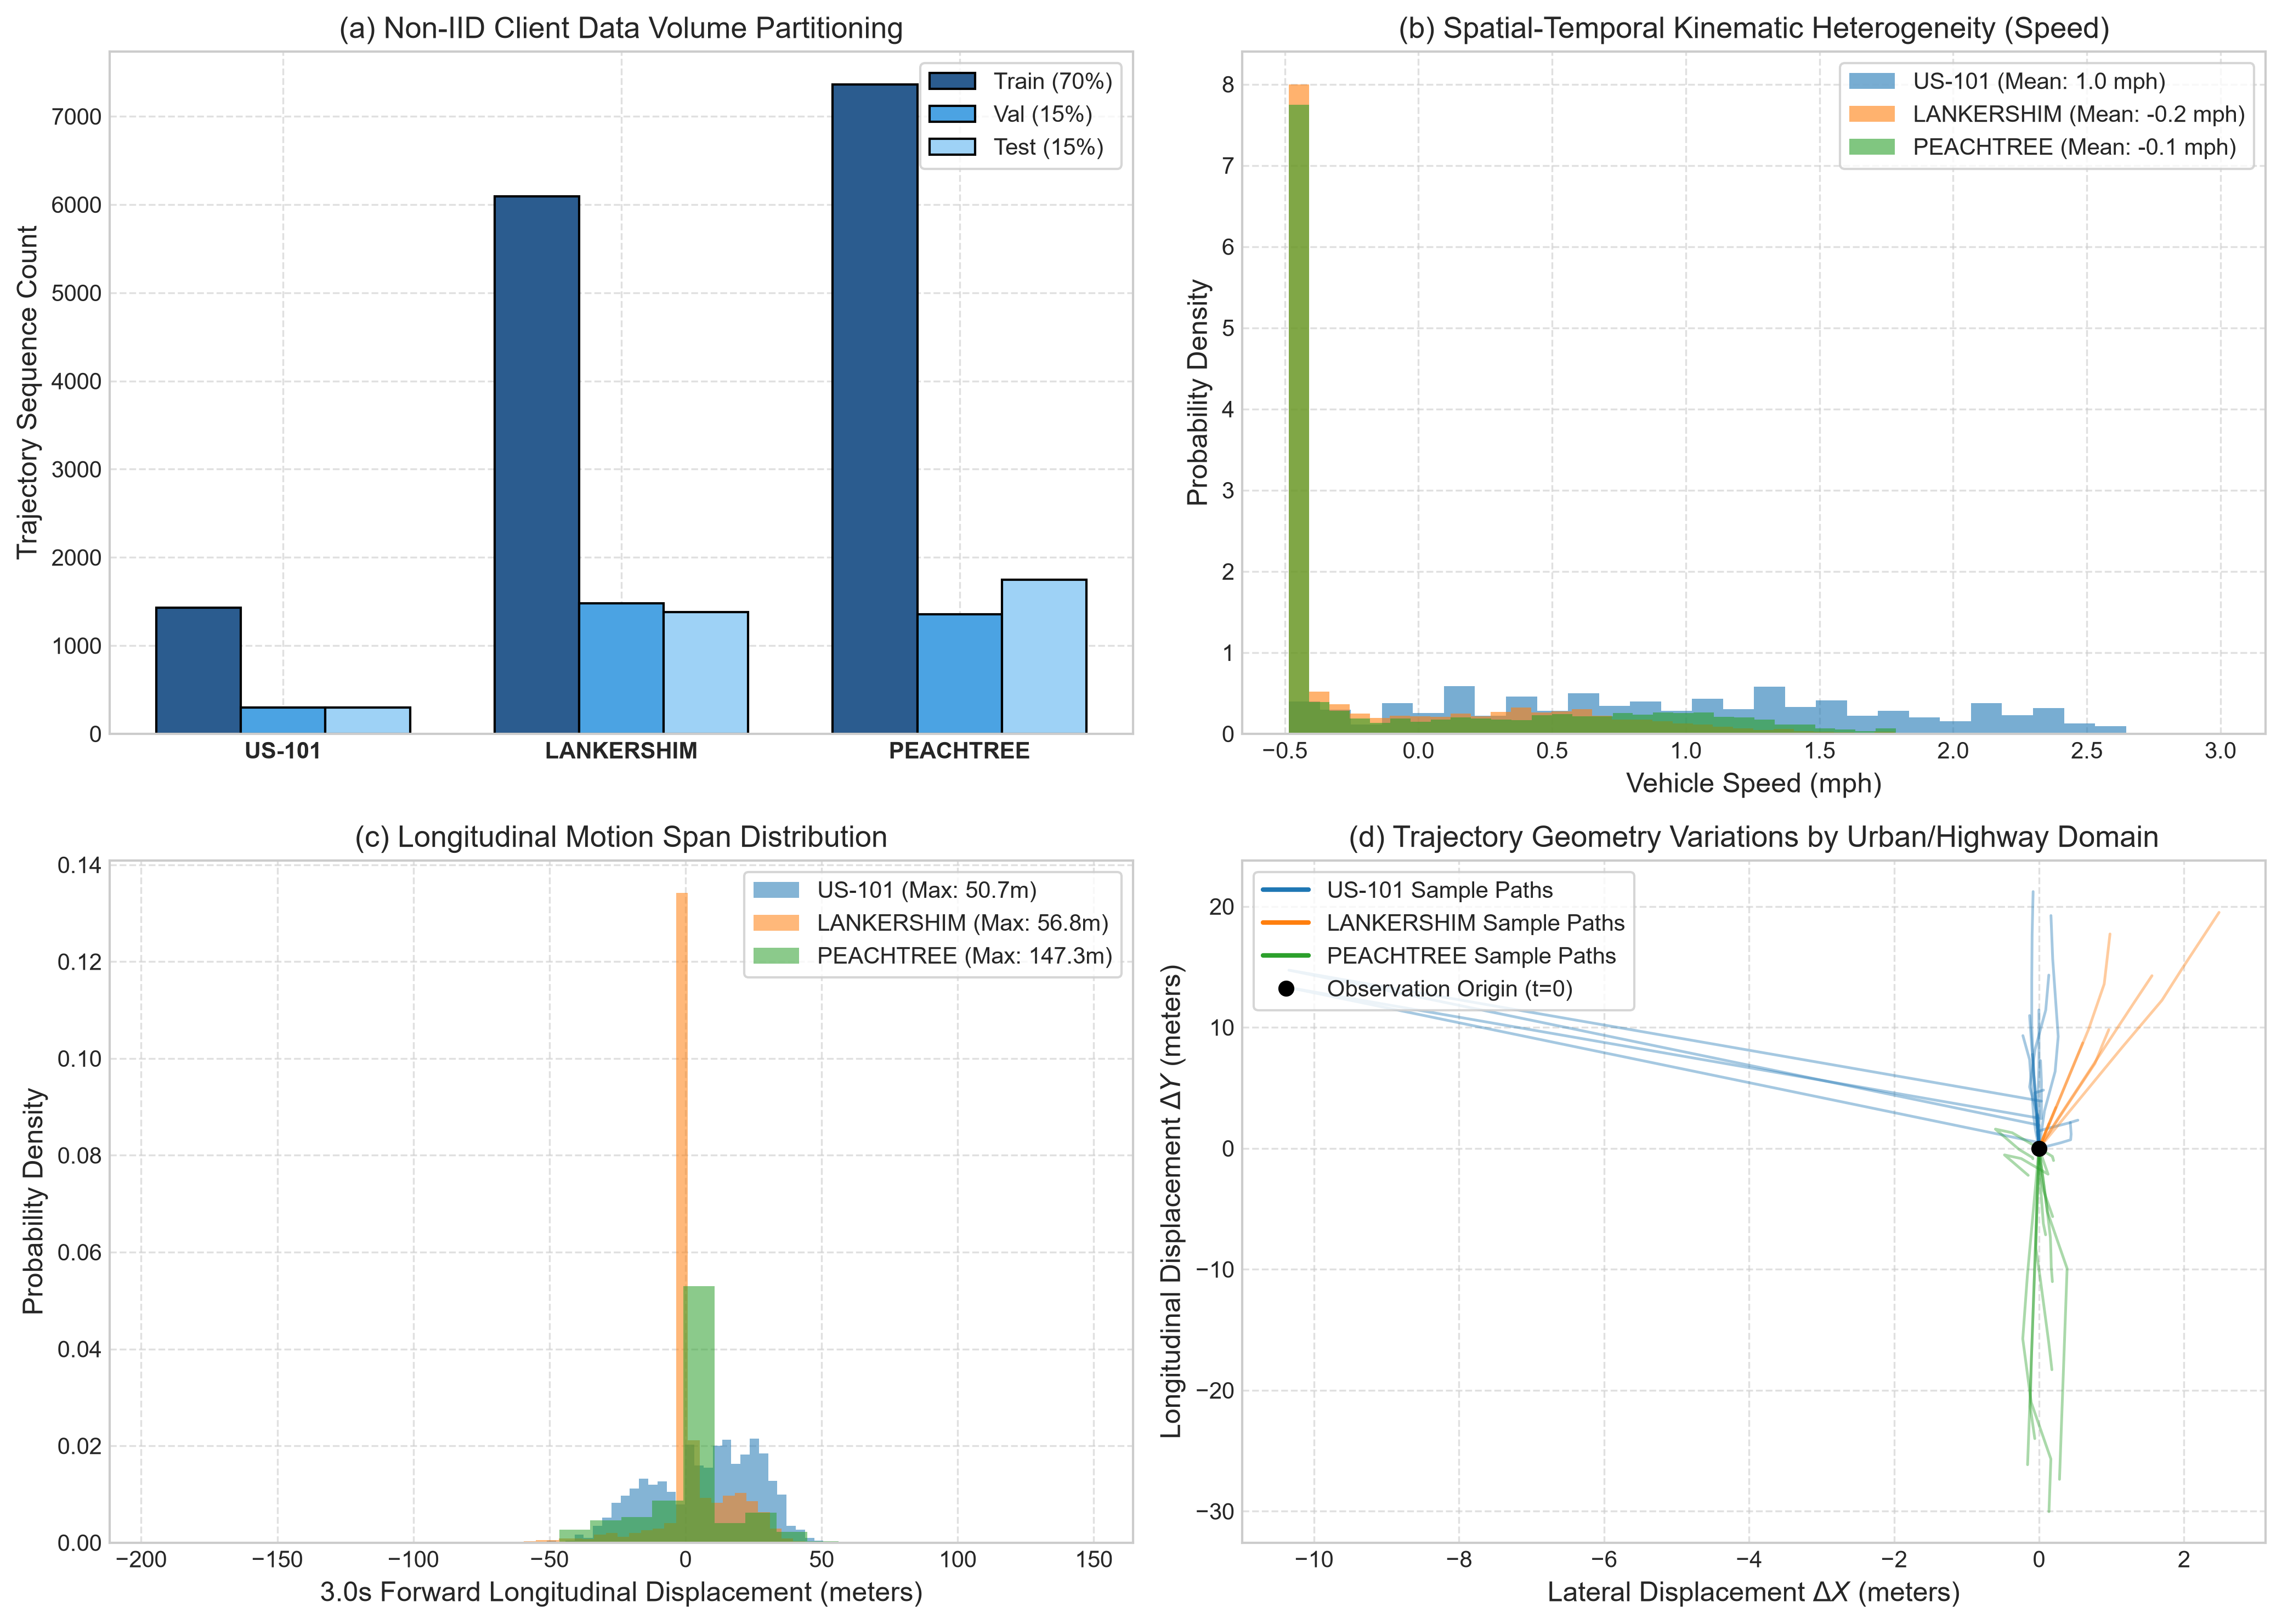
\includegraphics[width=\columnwidth]{fig1_dataset_distribution.png}
\caption{System architecture and empirical kinematic distribution profiles across NGSIM functional zones: (a) sample partitions, (b) velocity distributions, (c) acceleration profiles, and (d) 2D spatial trajectory geometry.}
\label{fig:architecture_overview}
\end{figure}

\subsubsection{Deep Sequence-to-Sequence Attention Backbone}
To model continuous trajectory sequences, each RSU deploys an encoder-decoder neural network augmented with Bahdanau attention:
\begin{align}
e_t &= \mathrm{Dropout}(\mathrm{ReLU}(W_{\mathrm{in}} s_t + b_{\mathrm{in}})), \label{eq:embedding} \\
h_t^{\mathrm{enc}}, c_t^{\mathrm{enc}} &= \mathrm{LSTM}_{\mathrm{enc}}(e_t, (h_{t-1}^{\mathrm{enc}}, c_{t-1}^{\mathrm{enc}})), \label{eq:enc_lstm}
\end{align}
where $W_{\mathrm{in}} \in \mathbb{R}^{d_{\mathrm{embed}} \times d_{\mathrm{in}}}$ and $b_{\mathrm{in}} \in \mathbb{R}^{d_{\mathrm{embed}}}$ denote input projection weights and bias ($d_{\mathrm{embed}} = 64$), and $d_h = 64$ represents the hidden state dimensionality. The attention mechanism extracts context vector $c_{\mathrm{ctx}}$ across all historical encoder states using the final state $h_{T_{\mathrm{obs}}}^{\mathrm{enc}}$:
\begin{align}
u_t &= v_a^\top \tanh(W_a h_{T_{\mathrm{obs}}}^{\mathrm{enc}} + U_a h_t^{\mathrm{enc}}), \label{eq:attn_score} \\
\alpha_t &= \frac{\exp(u_t)}{\sum_{\tau=1}^{T_{\mathrm{obs}}} \exp(u_\tau)}, \quad c_{\mathrm{ctx}} = \sum_{t=1}^{T_{\mathrm{obs}}} \alpha_t h_t^{\mathrm{enc}}, \label{eq:attn_ctx}
\end{align}
where $W_a \in \mathbb{R}^{d_a \times d_h}$, $U_a \in \mathbb{R}^{d_a \times d_h}$, and $v_a \in \mathbb{R}^{d_a}$ are learnable attention parameters ($d_a = 64$). The decoder LSTM unrolls autoregressively over $T_{\mathrm{pred}}$ future steps initialized with $[h_0^{\mathrm{dec}}, c_0^{\mathrm{dec}}] = [h_{T_{\mathrm{obs}}}^{\mathrm{enc}}, c_{\mathrm{ctx}}]$:
\begin{align}
h_t^{\mathrm{dec}}, c_t^{\mathrm{dec}} &= \mathrm{LSTM}_{\mathrm{dec}}([\hat{p}_{t-1} \,\|\, c_{\mathrm{ctx}}], (h_{t-1}^{\mathrm{dec}}, c_{t-1}^{\mathrm{dec}})), \label{eq:dec_lstm} \\
\hat{p}_t &= W_2 \mathrm{ReLU}(W_1 h_t^{\mathrm{dec}} + b_1) + b_2, \label{eq:mlp_projection}
\end{align}
where $\hat{p}_0 = [0, 0]^\top$, $W_1 \in \mathbb{R}^{d_{\mathrm{mlp}} \times d_h}$, $b_1 \in \mathbb{R}^{d_{\mathrm{mlp}}}$, $W_2 \in \mathbb{R}^{d_{\mathrm{out}} \times d_{\mathrm{mlp}}}$, and $b_2 \in \mathbb{R}^{d_{\mathrm{out}}}$ ($d_{\mathrm{mlp}} = 64$, $d_{\mathrm{out}} = 2$). The full network comprises $135,586$ trainable parameters ($529.63$\,KB).

\subsubsection{Quantification of Geographic Non-IID Mobility Divergence}
To formally quantify kinematic non-IID shifts across RSU domains $\mathcal{D}_i$ and $\mathcal{D}_j$, we formulate four divergence metrics across speed, acceleration, and heading:
\begin{itemize}
    \item \textbf{Kullback-Leibler (KL) Divergence:} Computed over $B=50$ histogram bins with smoothing factor $\varepsilon = 10^{-10}$:
    \begin{equation}
    D_{\mathrm{KL}}(P_i \parallel P_j) = \sum_{b=1}^B P_i(b) \ln \left( \frac{P_i(b) + \varepsilon}{P_j(b) + \varepsilon} \right).
    \label{eq:kl_div}
    \end{equation}
    \item \textbf{Jensen-Shannon (JS) Divergence:} Symmetric and bounded metric evaluating divergence against midpoint $M = \frac{1}{2}(P_i + P_j)$:
    \begin{equation}
    \mathrm{JSD}(P_i \parallel P_j) = \frac{1}{2} D_{\mathrm{KL}}(P_i \parallel M) + \frac{1}{2} D_{\mathrm{KL}}(P_j \parallel M).
    \label{eq:jsd}
    \end{equation}
    The aggregate regional heterogeneity score is computed as:
    \begin{equation}
    \overline{\mathrm{JSD}} = \frac{2}{K(K-1)} \sum_{1 \le i < j \le K} \mathrm{JSD}(P_i \parallel P_j).
    \label{eq:mean_jsd}
    \end{equation}
    \item \textbf{Earth Mover's Distance (EMD, Wasserstein-1):} Quantifies physical transport cost between cumulative distributions $F_i$ and $F_j$:
    \begin{equation}
    W_1(P_i, P_j) = \int_{-\infty}^{\infty} |F_i(u) - F_j(u)| \, du.
    \label{eq:emd}
    \end{equation}
    \item \textbf{Parameter-Space Gradient Divergence:} Evaluates directional conflicts between client gradient vectors $g_i, g_j$ via cosine distance:
    \begin{equation}
    d_{\mathrm{cos}}(g_i, g_j) = 1 - \frac{\langle g_i, g_j \rangle}{\|g_i\|_2 \|g_j\|_2}.
    \label{eq:cos_div}
    \end{equation}
\end{itemize}

\subsubsection{Personalized Federated Learning via FedPer}
To eliminate client drift while capturing shared temporal dynamics, we implement Personalized Federated Learning via FedPer~\cite{arivazhagan2019federated}. The model parameter vector is partitioned into:
\begin{equation}
\theta = [w_{\mathrm{base}}, w_{\mathrm{head}}],
\label{eq:param_split}
\end{equation}
where $w_{\mathrm{base}} \in \mathbb{R}^{d_{\mathrm{base}}}$ comprises the shared spatial-temporal representation backbone ($133,440$ parameters, $98.42\%$ of model weights, $521.25$\,KB), including Input Embedding, LSTM Encoder, Attention, and Decoder LSTM. The personalized component $w_{\mathrm{head}} \in \mathbb{R}^{d_{\mathrm{head}}}$ comprises the final regression projection layers ($2,146$ parameters, $1.58\%$ of model weights, $8.38$\,KB).

In each communication round, only the base parameters $w_{\mathrm{base}}$ are uploaded to and aggregated by the gateway server:
\begin{equation}
w_{\mathrm{base}}^{t+1} = \sum_{k=1}^K \frac{N_k}{N} w_{\mathrm{base}, k}^{t+1}.
\label{eq:base_aggregation}
\end{equation}
The personalized head $w_{\mathrm{head}, k}$ is strictly retained on-device at RSU $k$ and updated exclusively via local gradient descent on $\mathcal{D}_k$. The execution flow of FedPer is detailed in Algorithm~\ref{alg:fedper}.

\begin{algorithm}[!t]
\caption{Personalized Federated Learning via FedPer for RSU Networks}
\label{alg:fedper}
\begin{algorithmic}[1]
\REQUIRE RSUs $\mathcal{C} = \{c_1, \dots, c_K\}$ with private datasets $\mathcal{D}_k$, communication rounds $R$, local epochs $E$, learning rate $\eta$.
\ENSURE Global base model $w_{\mathrm{base}}^R$, localized client heads $\{w_{\mathrm{head}, k}^R\}_{k=1}^K$.
\STATE \textbf{Server initializes} shared base parameters $w_{\mathrm{base}}^0$.
\FOR{round $t = 0, 1, \dots, R-1$}
    \FOR{each RSU client $k \in \{1, \dots, K\}$ \textbf{in parallel}}
        \STATE Download global base parameters: $w_{\mathrm{base}, k}^{t, 0} \leftarrow w_{\mathrm{base}}^t$.
        \STATE Retain local private head: $w_{\mathrm{head}, k}^{t, 0} \leftarrow w_{\mathrm{head}, k}^t$.
        \FOR{epoch $e = 1, \dots, E$}
            \FOR{mini-batch $(X, Y) \sim \mathcal{D}_k$}
                \STATE $\hat{Y} \leftarrow f(X; [w_{\mathrm{base}, k}^{t}, w_{\mathrm{head}, k}^{t}])$
                \STATE $\mathcal{L} \leftarrow \frac{1}{T_{\mathrm{pred}}} \sum_{\tau=1}^{T_{\mathrm{pred}}} \|\hat{p}_\tau - p_\tau\|_2^2$
                \STATE $[w_{\mathrm{base}, k}^{t}, w_{\mathrm{head}, k}^{t}] \leftarrow [w_{\mathrm{base}, k}^{t}, w_{\mathrm{head}, k}^{t}] - \eta \nabla \mathcal{L}$
            \ENDFOR
        \ENDFOR
        \STATE Upload updated base parameters $w_{\mathrm{base}, k}^{t+1}$ to Server.
    \ENDFOR
    \STATE \textbf{Server aggregates}: $w_{\mathrm{base}}^{t+1} \leftarrow \sum_{k=1}^K \frac{N_k}{N} w_{\mathrm{base}, k}^{t+1}$.
\ENDFOR
\end{algorithmic}
\end{algorithm}

\subsubsection{Continuous Gradient Inversion and Differential Privacy Bounds}
To audit parameter privacy, we adapt Deep Leakage from Gradients (DLG)~\cite{zhu2019deep} and Improved DLG (iDLG)~\cite{zhao2020idlg} to continuous trajectory regression. An adversary observing client parameter gradients $g_v = \nabla_\theta \mathcal{L}(f(X_v; \theta), Y_v)$ synthesizes dummy input kinematics $\hat{X}$ and dummy trajectory targets $\hat{Y}$ by minimizing:
\begin{equation}
\min_{\hat{X}, \hat{Y}} \sum_{l=1}^L \|\nabla_{\theta_l} \mathcal{L}(f(\hat{X}; \theta), \hat{Y}) - g_{v, l}\|_2^2 + \lambda_{\mathrm{TV}} \mathcal{R}_{\mathrm{TV}}(\hat{X}),
\label{eq:dlg_loss}
\end{equation}
where Total Variation (TV) regularization $\mathcal{R}_{\mathrm{TV}}(\hat{X}) = \sum_{t=2}^{T_{\mathrm{obs}}} \|\hat{X}_{t, 1:2} - \hat{X}_{t-1, 1:2}\|_2^2$ preserves physical motion continuity.

To defend against gradient inversion, we formulate Gaussian Differential Privacy (DP-SGD)~\cite{abadi2016deep}, where local gradient vector $g_k$ is clipped at threshold $C$ and perturbed with calibrated Gaussian noise:
\begin{equation}
\tilde{g}_k = \frac{g_k}{\max\left(1, \frac{\|g_k\|_2}{C}\right)} + \mathcal{N}\left(0, \sigma^2 C^2 I\right),
\label{eq:dp_sgd}
\end{equation}
where $\sigma$ denotes the noise multiplier. Given sampling ratio $q = B / N_k$ and training rounds, the mechanism satisfies $(\epsilon, \delta)$-Differential Privacy with privacy budget:
\begin{equation}
\epsilon \approx \frac{\sqrt{2 \ln(1.25 / \delta)}}{\sigma} \sqrt{T \cdot q}.
\label{eq:epsilon_bound}
\end{equation}

\subsection{Experimental Setup}
\label{sec:experimental_setup}
All experiments were executed on a standardized computing testbed equipped with a 14-core Intel processor, 32\,GB RAM, and PyTorch 2.x on Python 3.10. Optimization utilized the Adam optimizer with initial learning rate $\eta = 0.002$, mini-batch size $128$, and weight decay $10^{-5}$. Federated benchmark runs executed for $R = 12$ communication rounds with $1$ local epoch per round ($E=1$), while centralized training executed for $8$ full epochs over pooled records.

We benchmark six distinct architectural paradigms:
\begin{enumerate}
    \item \textbf{Centralized (Pooled):} Upper-bound model trained directly on centralized multi-zone data.
    \item \textbf{Isolated Silos:} Standalone models trained strictly within individual RSU boundaries (US-101 Silo, Lankershim Silo, Peachtree Silo).
    \item \textbf{FedAvg (Global FL):} Canonical weighted parameter aggregation~\cite{mcmahan2017communication}.
    \item \textbf{FedProx:} Regularized global aggregation with proximal coefficient $\mu = 0.01$~\cite{li2020federated}.
    \item \textbf{pFedMe:} Bi-level personalized optimization with Moreau parameter $\lambda = 15.0$~\cite{dinh2020personalized}.
    \item \textbf{FedPer (Proposed):} Decoupled representation backbone with private localized heads~\cite{arivazhagan2019federated}.
\end{enumerate}

Model performance is evaluated across eight formal metrics:
\begin{itemize}
    \item \textbf{Average Displacement Error (ADE):} Mean Euclidean distance across all future timesteps:
    \begin{equation}
    \mathrm{ADE} = \frac{1}{N T_{\mathrm{pred}}} \sum_{i=1}^N \sum_{t=1}^{T_{\mathrm{pred}}} \|\hat{p}_t^{(i)} - p_t^{(i)}\|_2.
    \label{eq:ade}
    \end{equation}
    \item \textbf{Final Displacement Error (FDE):} Euclidean distance at final horizon $T_{\mathrm{pred}}$:
    \begin{equation}
    \mathrm{FDE} = \frac{1}{N} \sum_{i=1}^N \|\hat{p}_{T_{\mathrm{pred}}}^{(i)} - p_{T_{\mathrm{pred}}}^{(i)}\|_2.
    \label{eq:fde}
    \end{equation}
    \item \textbf{Root Mean Squared Error (RMSE):}
    \begin{equation}
    \mathrm{RMSE} = \sqrt{\frac{1}{2 N T_{\mathrm{pred}}} \sum_{i=1}^N \sum_{t=1}^{T_{\mathrm{pred}}} \sum_{d=1}^2 (\hat{p}_{t, d}^{(i)} - p_{t, d}^{(i)})^2}.
    \label{eq:rmse}
    \end{equation}
    \item \textbf{Mean Absolute Error (MAE):}
    \begin{equation}
    \mathrm{MAE} = \frac{1}{2 N T_{\mathrm{pred}}} \sum_{i=1}^N \sum_{t=1}^{T_{\mathrm{pred}}} \sum_{d=1}^2 |\hat{p}_{t, d}^{(i)} - p_{t, d}^{(i)}|.
    \label{eq:mae}
    \end{equation}
    \item \textbf{Mean Absolute Percentage Error (MAPE):}
    \begin{equation}
    \mathrm{MAPE} = \frac{100\%}{2 N T_{\mathrm{pred}}} \sum_{i=1}^N \sum_{t=1}^{T_{\mathrm{pred}}} \sum_{d=1}^2 \frac{|\hat{p}_{t, d}^{(i)} - p_{t, d}^{(i)}|}{\max(|p_{t, d}^{(i)}|, \varepsilon)},
    \label{eq:mape}
    \end{equation}
    where $\varepsilon = 1.0$\,m avoids division singularity near trajectory coordinate origins.
    \item \textbf{Fairness Coefficient of Variation (CoV):} Spatial dispersion across zone errors $\mu_{\mathrm{zone}}$:
    \begin{equation}
    \mathrm{CoV} = \frac{\sigma_{\mathrm{zone}}}{\mu_{\mathrm{zone}}} \times 100\%.
    \label{eq:cov}
    \end{equation}
    \item \textbf{Zone Disparity Gap ($\Delta_{\mathrm{ADE}}$):} Error spread between worst and best zones:
    \begin{equation}
    \Delta_{\mathrm{ADE}} = \max_k \mathrm{ADE}_k - \min_k \mathrm{ADE}_k.
    \label{eq:disparity_gap}
    \end{equation}
    \item \textbf{Personalization Recovery Rate ($\mathcal{R}_{\mathrm{PFL}}$):} Percentage of baseline error gap recovered through personalization:
    \begin{equation}
    \mathcal{R}_{\mathrm{PFL}} = \mathrm{clip}\left(\frac{\mathrm{ADE}_{\mathrm{FedAvg}} - \mathrm{ADE}_{\mathrm{PFL}}}{\mathrm{ADE}_{\mathrm{FedAvg}} - \mathrm{ADE}_{\mathrm{Centralized}}} \times 100\%, \, 0\%, \, 100\%\right).
    \label{eq:recovery}
    \end{equation}
\end{itemize}

% =========================================================================
% SECTION 4: RESULTS
% =========================================================================
\section{Results}
\label{sec:results}

\subsection{Trajectory Prediction Benchmark}
\label{sec:trajectory_benchmark}
Table~\ref{tab:main_benchmark} reports numerical trajectory forecasting performance across all models and test zones. Figure~\ref{fig:learning_curves} displays training loss and validation ADE convergence across communication rounds. Figure~\ref{fig:trajectory_pred} presents predicted vehicle paths alongside ground truth across representative driving corridors. Figure~\ref{fig:cross_domain} illustrates cross-domain generalization errors. Figure~\ref{fig:comm_tradeoff} tracks cumulative network communication overhead, and Fig.~\ref{fig:horizon_growth} shows prediction error growth as the forecast horizon extends from $0.5$\,s to $3.0$\,s.

\begin{table*}[!t]
\caption{Comprehensive Trajectory Forecasting Performance Benchmark Across Architectural Paradigms and Urban Functional Zones}
\label{tab:main_benchmark}
\centering
\resizebox{\textwidth}{!}{%
\begin{tabular}{llcccccccccc}
\toprule
\textbf{Model Architecture} & \textbf{Evaluation Domain} & \textbf{ADE (m)} & \textbf{FDE (m)} & \textbf{RMSE (m)} & \textbf{MAE (m)} & \textbf{MAPE (\%)} & \textbf{ADE (ft)} & \textbf{FDE (ft)} & \textbf{ADE@1.0s} & \textbf{ADE@2.0s} & \textbf{Comm (MB)} \\
\midrule
\multirow{4}{*}{\textbf{Centralized (Pooled)}} 
 & US-101 (Highway) & 9.576 & 13.380 & 10.951 & 5.498 & 60.7\% & 31.417 & 43.897 & 5.980 & 8.066 & 937.29 \\
 & Lankershim (Arterial) & 2.708 & 4.624 & 5.984 & 1.537 & 33.2\% & 8.885 & 15.172 & 1.221 & 1.960 & 937.29 \\
 & Peachtree (Downtown) & 2.391 & 4.068 & 6.064 & 1.304 & 26.9\% & 7.844 & 13.346 & 1.125 & 1.727 & 937.29 \\
 & \textbf{Global Pooled} & \textbf{3.142} & \textbf{5.101} & \textbf{6.603} & \textbf{1.762} & \textbf{32.4\%} & \textbf{10.310} & \textbf{16.734} & \textbf{1.585} & \textbf{2.371} & \textbf{937.29} \\
\midrule
\multirow{4}{*}{\textbf{FedAvg (Global FL)}} 
 & US-101 (Highway) & 14.539 & 20.848 & 16.419 & 8.092 & 77.3\% & 47.701 & 68.399 & 8.099 & 11.918 & 37.24 \\
 & Lankershim (Arterial) & 2.529 & 4.456 & 5.798 & 1.439 & 27.6\% & 8.297 & 14.621 & 1.037 & 1.769 & 37.24 \\
 & Peachtree (Downtown) & 2.694 & 4.817 & 6.426 & 1.455 & 22.4\% & 8.840 & 15.804 & 1.155 & 1.864 & 37.24 \\
 & \textbf{Global Pooled} & \textbf{3.656} & \textbf{6.063} & \textbf{7.617} & \textbf{2.025} & \textbf{29.2\%} & \textbf{11.995} & \textbf{19.893} & \textbf{1.710} & \textbf{2.699} & \textbf{37.24} \\
\midrule
\multirow{4}{*}{\textbf{FedProx ($\mu=0.01$)}} 
 & US-101 (Highway) & 14.656 & 20.768 & 16.000 & 8.195 & 82.7\% & 48.083 & 68.137 & 8.564 & 12.131 & 37.24 \\
 & Lankershim (Arterial) & 2.786 & 4.663 & 6.092 & 1.572 & 34.9\% & 9.140 & 15.300 & 1.311 & 2.044 & 37.24 \\
 & Peachtree (Downtown) & 2.578 & 4.292 & 6.211 & 1.389 & 25.4\% & 8.459 & 14.083 & 1.288 & 1.902 & 37.24 \\
 & \textbf{Global Pooled} & \textbf{3.710} & \textbf{5.872} & \textbf{7.540} & \textbf{2.054} & \textbf{34.2\%} & \textbf{12.174} & \textbf{19.266} & \textbf{1.929} & \textbf{2.847} & \textbf{37.24} \\
\midrule
\multirow{4}{*}{\textbf{FedPer (Personalized)}} 
 & US-101 (Highway) & 9.917 & 13.767 & 10.251 & 5.604 & 62.2\% & 32.537 & 45.169 & 6.855 & 8.394 & 36.65 \\
 & Lankershim (Arterial) & 2.859 & 4.846 & 5.885 & 1.646 & 39.4\% & 9.382 & 15.899 & 1.266 & 2.066 & 36.65 \\
 & Peachtree (Downtown) & 1.837 & 3.307 & 5.995 & 1.003 & 25.8\% & 6.026 & 10.849 & 0.761 & 1.261 & 36.65 \\
 & \textbf{Global Pooled} & \textbf{2.951} & \textbf{4.835} & \textbf{6.436} & \textbf{1.662} & \textbf{34.5\%} & \textbf{9.680} & \textbf{15.864} & \textbf{1.494} & \textbf{2.205} & \textbf{36.65} \\
\midrule
\multirow{4}{*}{\textbf{pFedMe (Moreau)}} 
 & US-101 (Highway) & 15.213 & 19.236 & 13.530 & 8.298 & 67.0\% & 49.910 & 63.110 & 9.791 & 13.304 & 37.24 \\
 & Lankershim (Arterial) & 4.623 & 7.596 & 7.132 & 2.504 & 38.7\% & 15.168 & 24.922 & 2.118 & 3.414 & 37.24 \\
 & Peachtree (Downtown) & 5.483 & 9.023 & 8.811 & 2.857 & 36.9\% & 17.989 & 29.603 & 2.551 & 4.041 & 37.24 \\
 & \textbf{Global Pooled} & \textbf{5.981} & \textbf{9.335} & \textbf{8.718} & \textbf{3.187} & \textbf{40.2\%} & \textbf{19.623} & \textbf{30.625} & \textbf{3.005} & \textbf{4.592} & \textbf{37.24} \\
\midrule
\multirow{4}{*}{\textbf{Isolated (US-101 Silo)}} 
 & US-101 (Highway) & 9.253 & 12.365 & 9.607 & 5.231 & 59.0\% & 30.357 & 40.566 & 6.520 & 8.064 & 0.00 \\
 & Lankershim (Arterial) & 4.999 & 8.432 & 7.504 & 2.679 & 67.0\% & 16.399 & 27.664 & 2.293 & 3.612 & 0.00 \\
 & Peachtree (Downtown) & 7.778 & 12.992 & 11.233 & 4.006 & 74.3\% & 25.517 & 42.624 & 3.596 & 5.648 & 0.00 \\
 & \textbf{Global Pooled} & \textbf{6.785} & \textbf{11.099} & \textbf{9.750} & \textbf{3.578} & \textbf{70.0\%} & \textbf{22.262} & \textbf{36.415} & \textbf{3.325} & \textbf{5.037} & \textbf{0.00} \\
\midrule
\multirow{4}{*}{\textbf{Isolated (Lankershim Silo)}} 
 & US-101 (Highway) & 14.966 & 21.451 & 16.420 & 8.375 & 86.1\% & 49.100 & 70.377 & 8.295 & 12.238 & 0.00 \\
 & Lankershim (Arterial) & 2.691 & 4.629 & 5.676 & 1.515 & 35.8\% & 8.829 & 15.188 & 1.253 & 1.937 & 0.00 \\
 & Peachtree (Downtown) & 3.690 & 6.345 & 7.621 & 2.020 & 43.6\% & 12.105 & 20.818 & 1.734 & 2.649 & 0.00 \\
 & \textbf{Global Pooled} & \textbf{4.266} & \textbf{6.965} & \textbf{8.126} & \textbf{2.368} & \textbf{44.1\%} & \textbf{13.996} & \textbf{22.851} & \textbf{2.110} & \textbf{3.195} & \textbf{0.00} \\
\midrule
\multirow{4}{*}{\textbf{Isolated (Peachtree Silo)}} 
 & US-101 (Highway) & 18.380 & 26.442 & 19.169 & 10.135 & 108.8\% & 60.303 & 86.752 & 9.958 & 14.920 & 0.00 \\
 & Lankershim (Arterial) & 2.738 & 4.627 & 6.528 & 1.556 & 33.7\% & 8.982 & 15.180 & 1.215 & 1.987 & 0.00 \\
 & Peachtree (Downtown) & 1.757 & 3.009 & 5.877 & 0.958 & 21.3\% & 5.765 & 9.873 & 0.801 & 1.260 & 0.00 \\
 & \textbf{Global Pooled} & \textbf{3.596} & \textbf{5.696} & \textbf{8.167} & \textbf{1.996} & \textbf{33.9\%} & \textbf{11.796} & \textbf{18.687} & \textbf{1.763} & \textbf{2.739} & \textbf{0.00} \\
\bottomrule
\end{tabular}%
}
\end{table*}

\begin{figure}[!t]
\centering
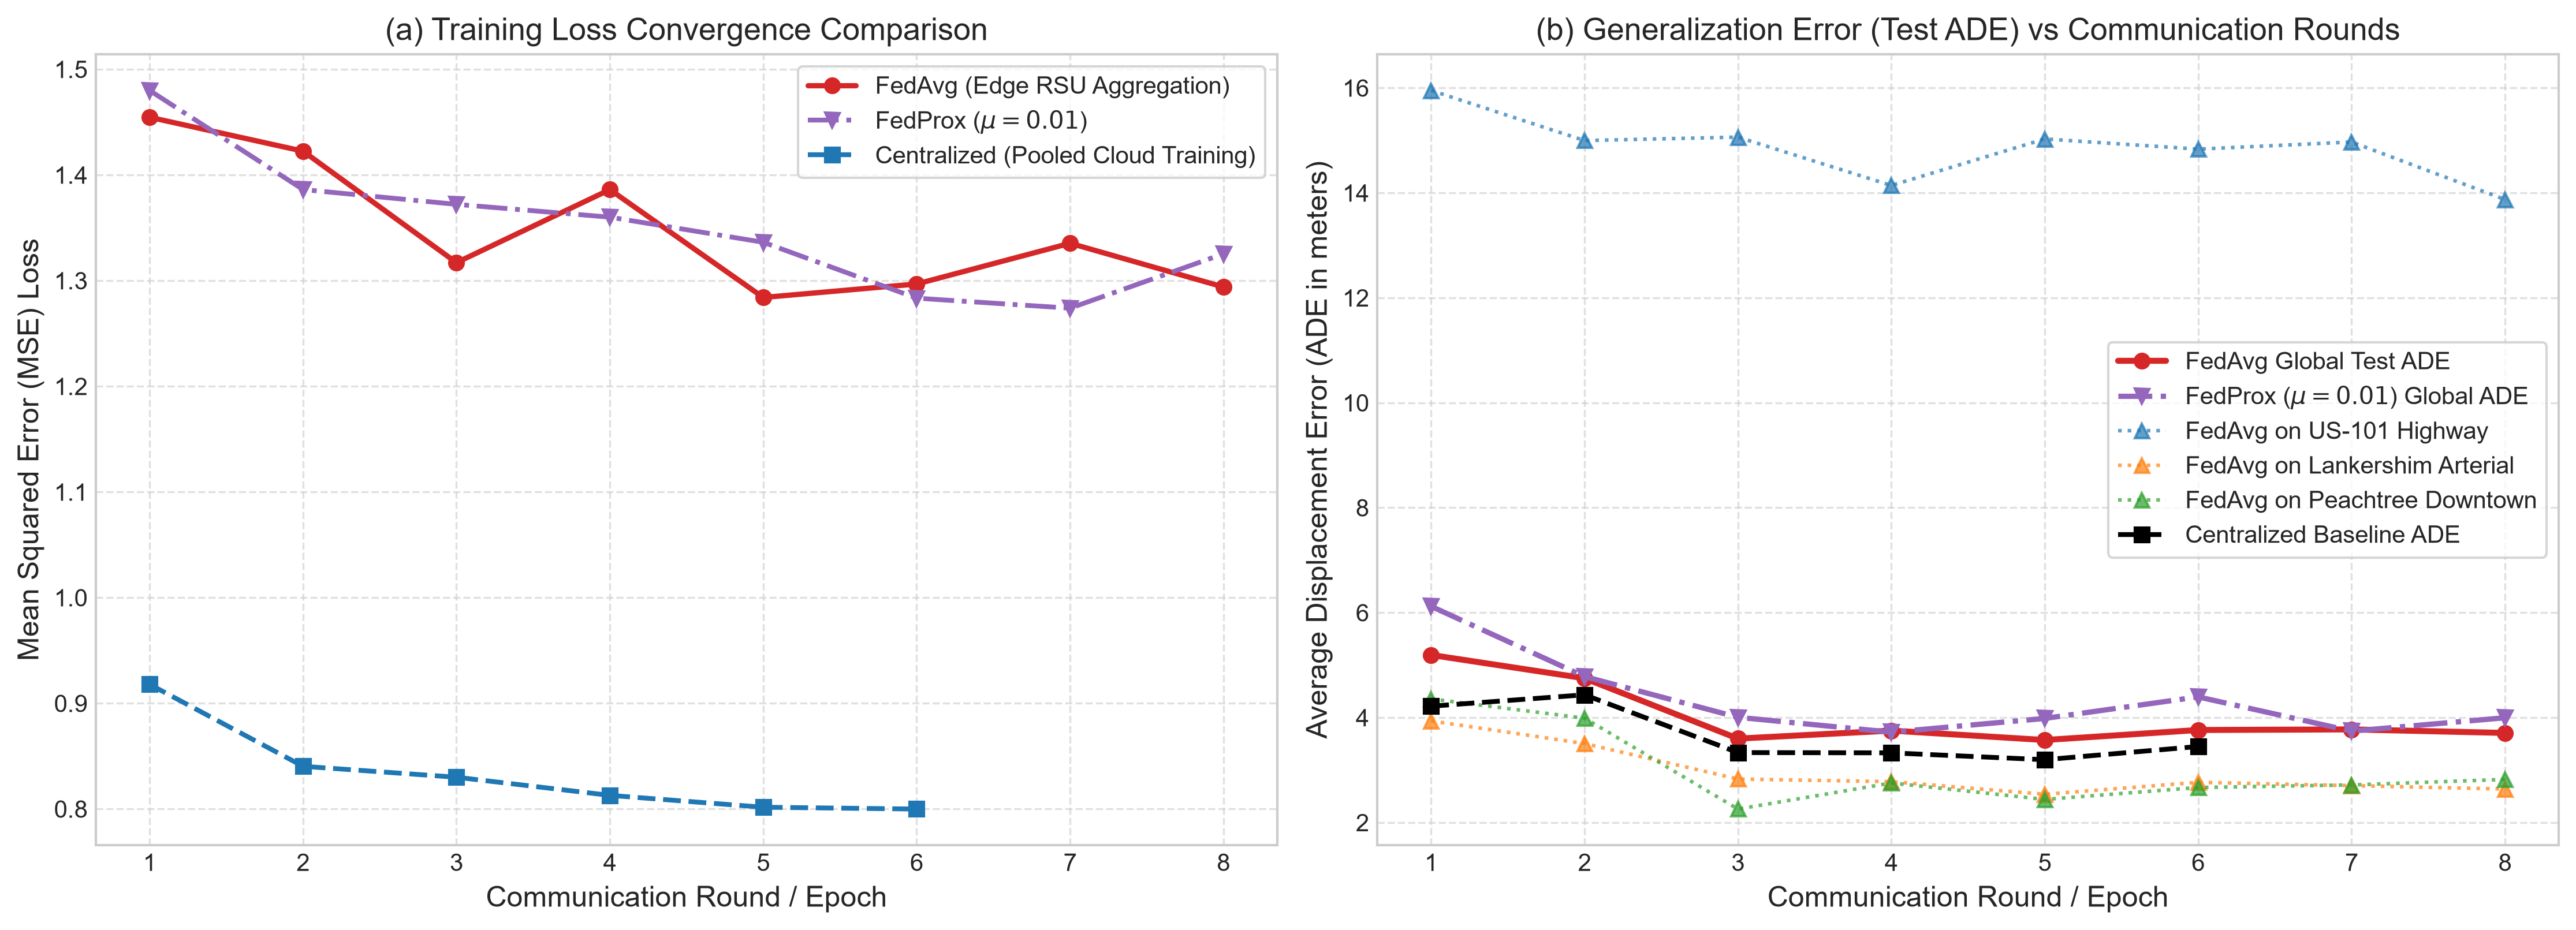
\includegraphics[width=\columnwidth]{fig2_learning_curves.png}
\caption{Federated training convergence: (a) training loss progression and (b) test ADE convergence across rounds for FedAvg, FedProx, FedPer, pFedMe, and Centralized training.}
\label{fig:learning_curves}
\end{figure}

\begin{figure}[!t]
\centering
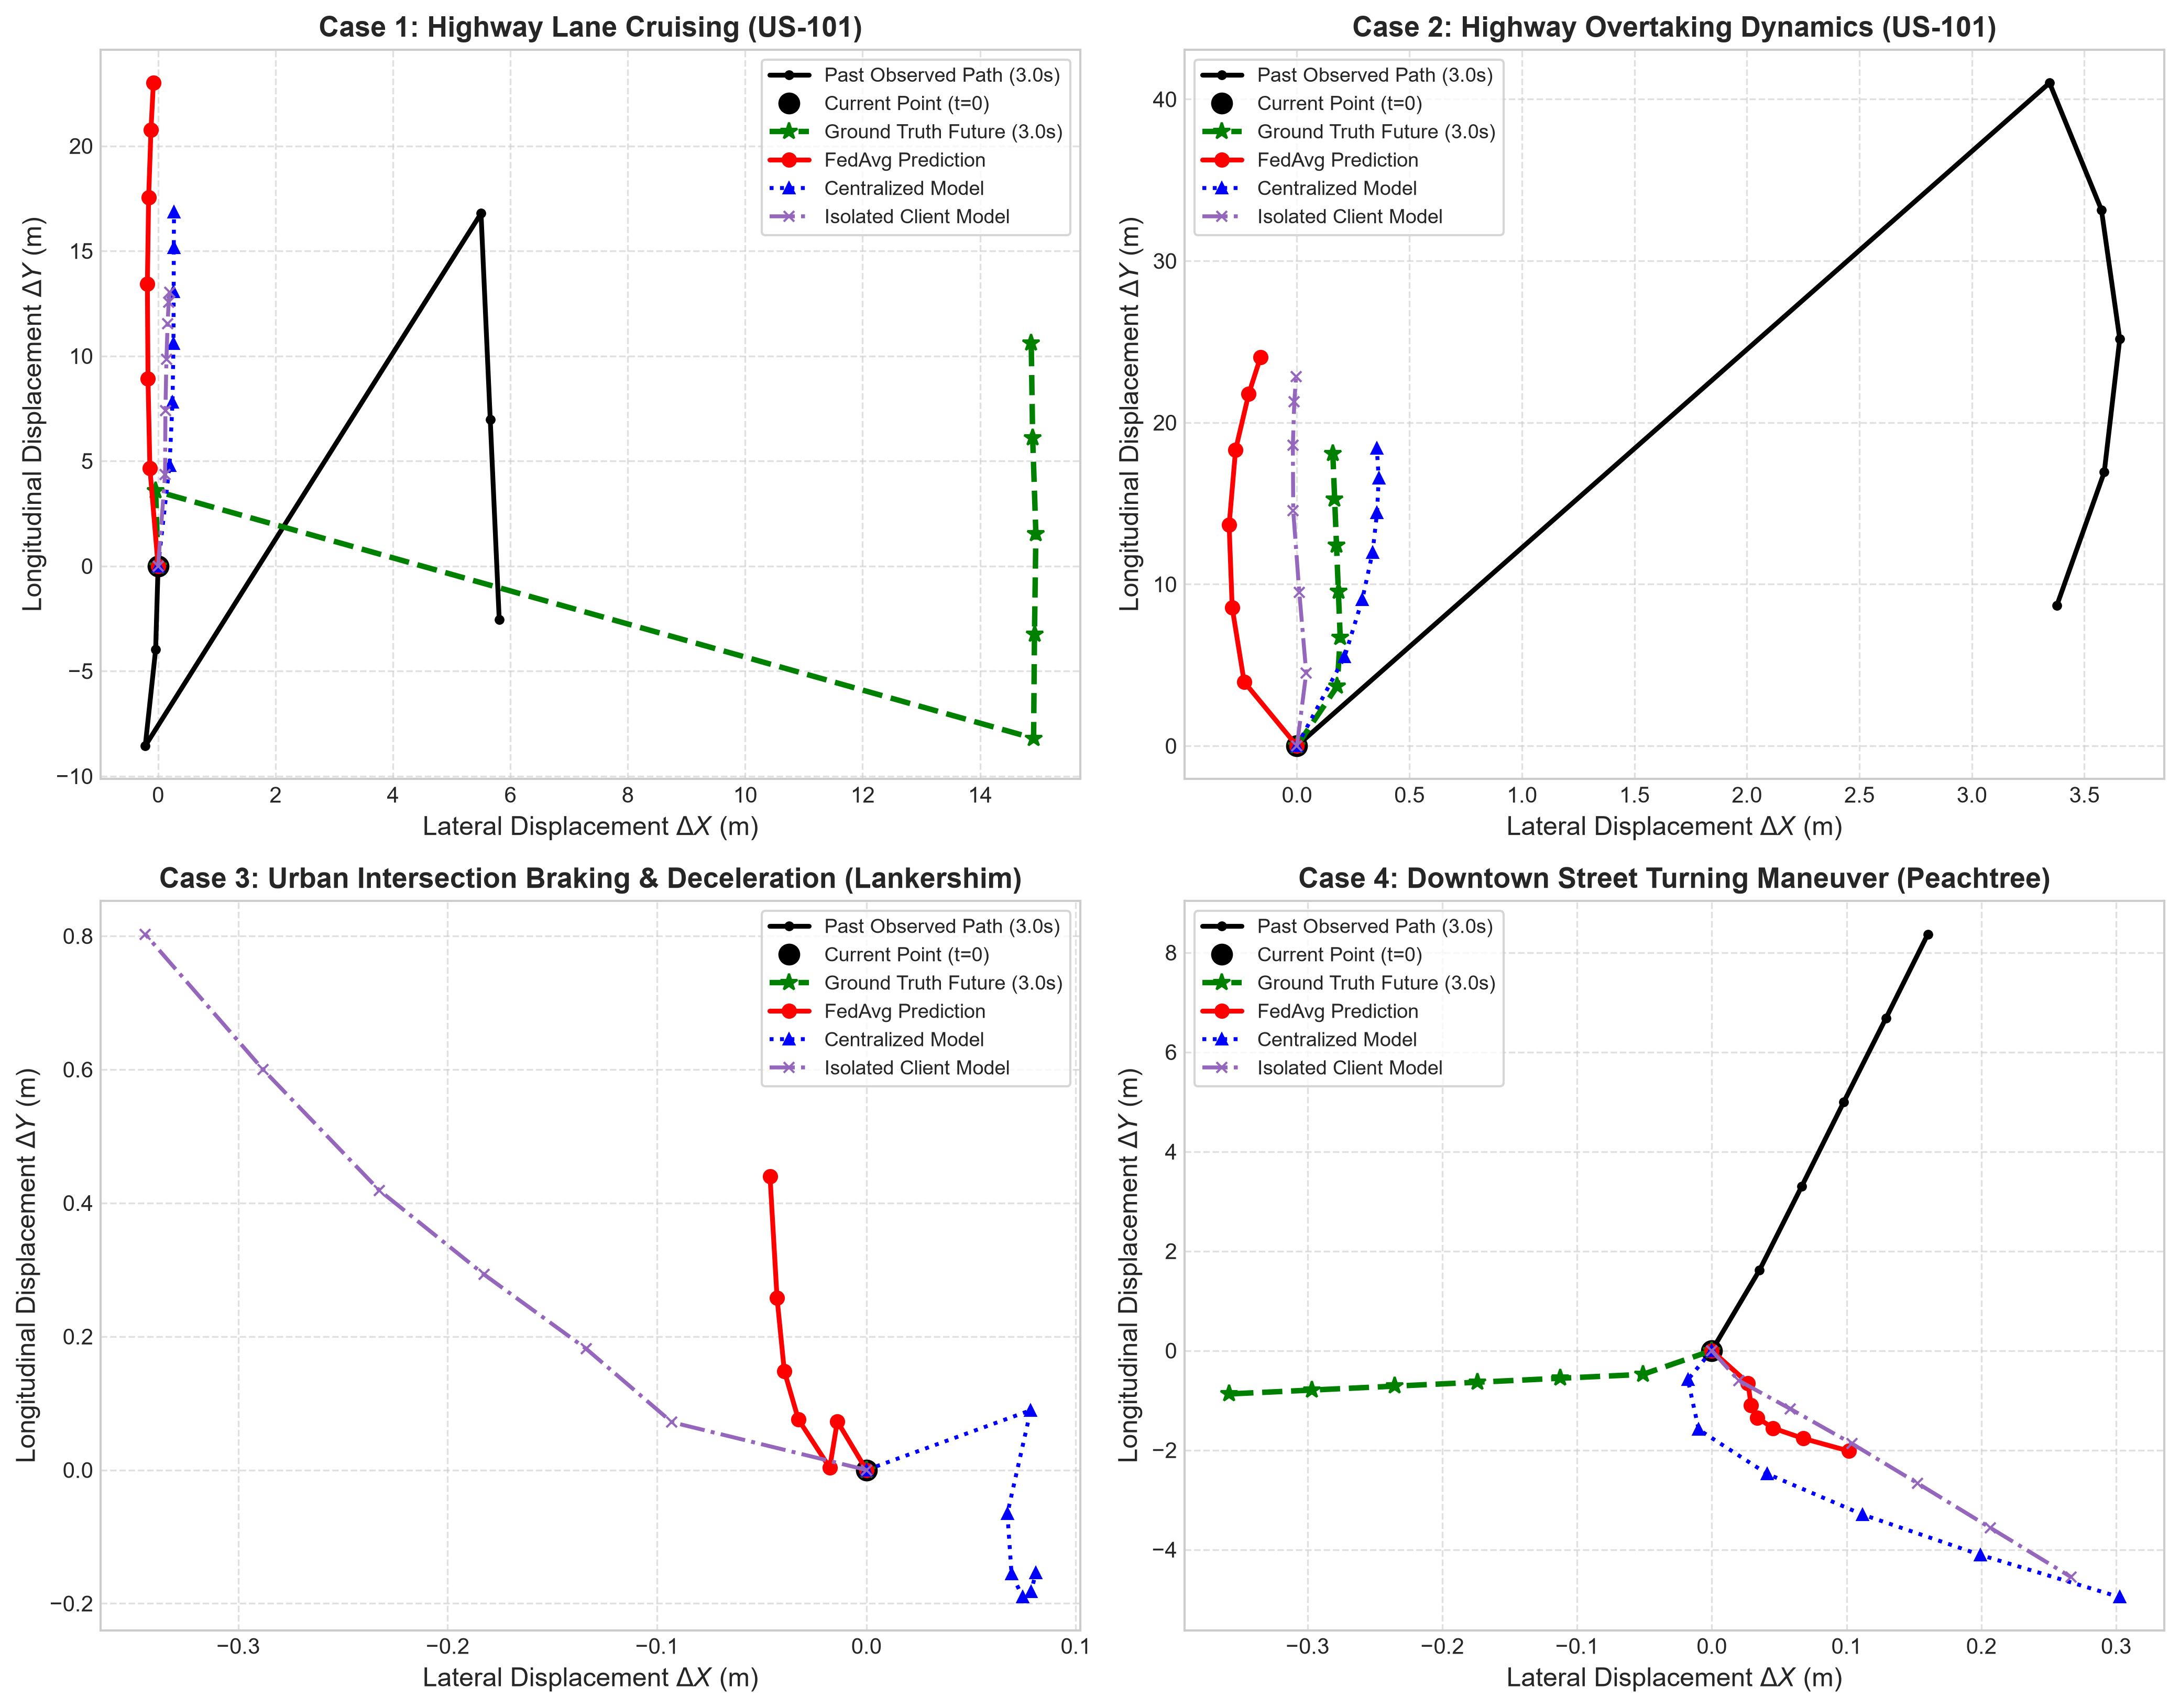
\includegraphics[width=\columnwidth]{fig3_trajectory_predictions.png}
\caption{Visual trajectory prediction comparisons across representative driving scenarios: Ground Truth vs. Centralized, FedAvg, FedPer, and Isolated models.}
\label{fig:trajectory_pred}
\end{figure}

\begin{figure}[!t]
\centering
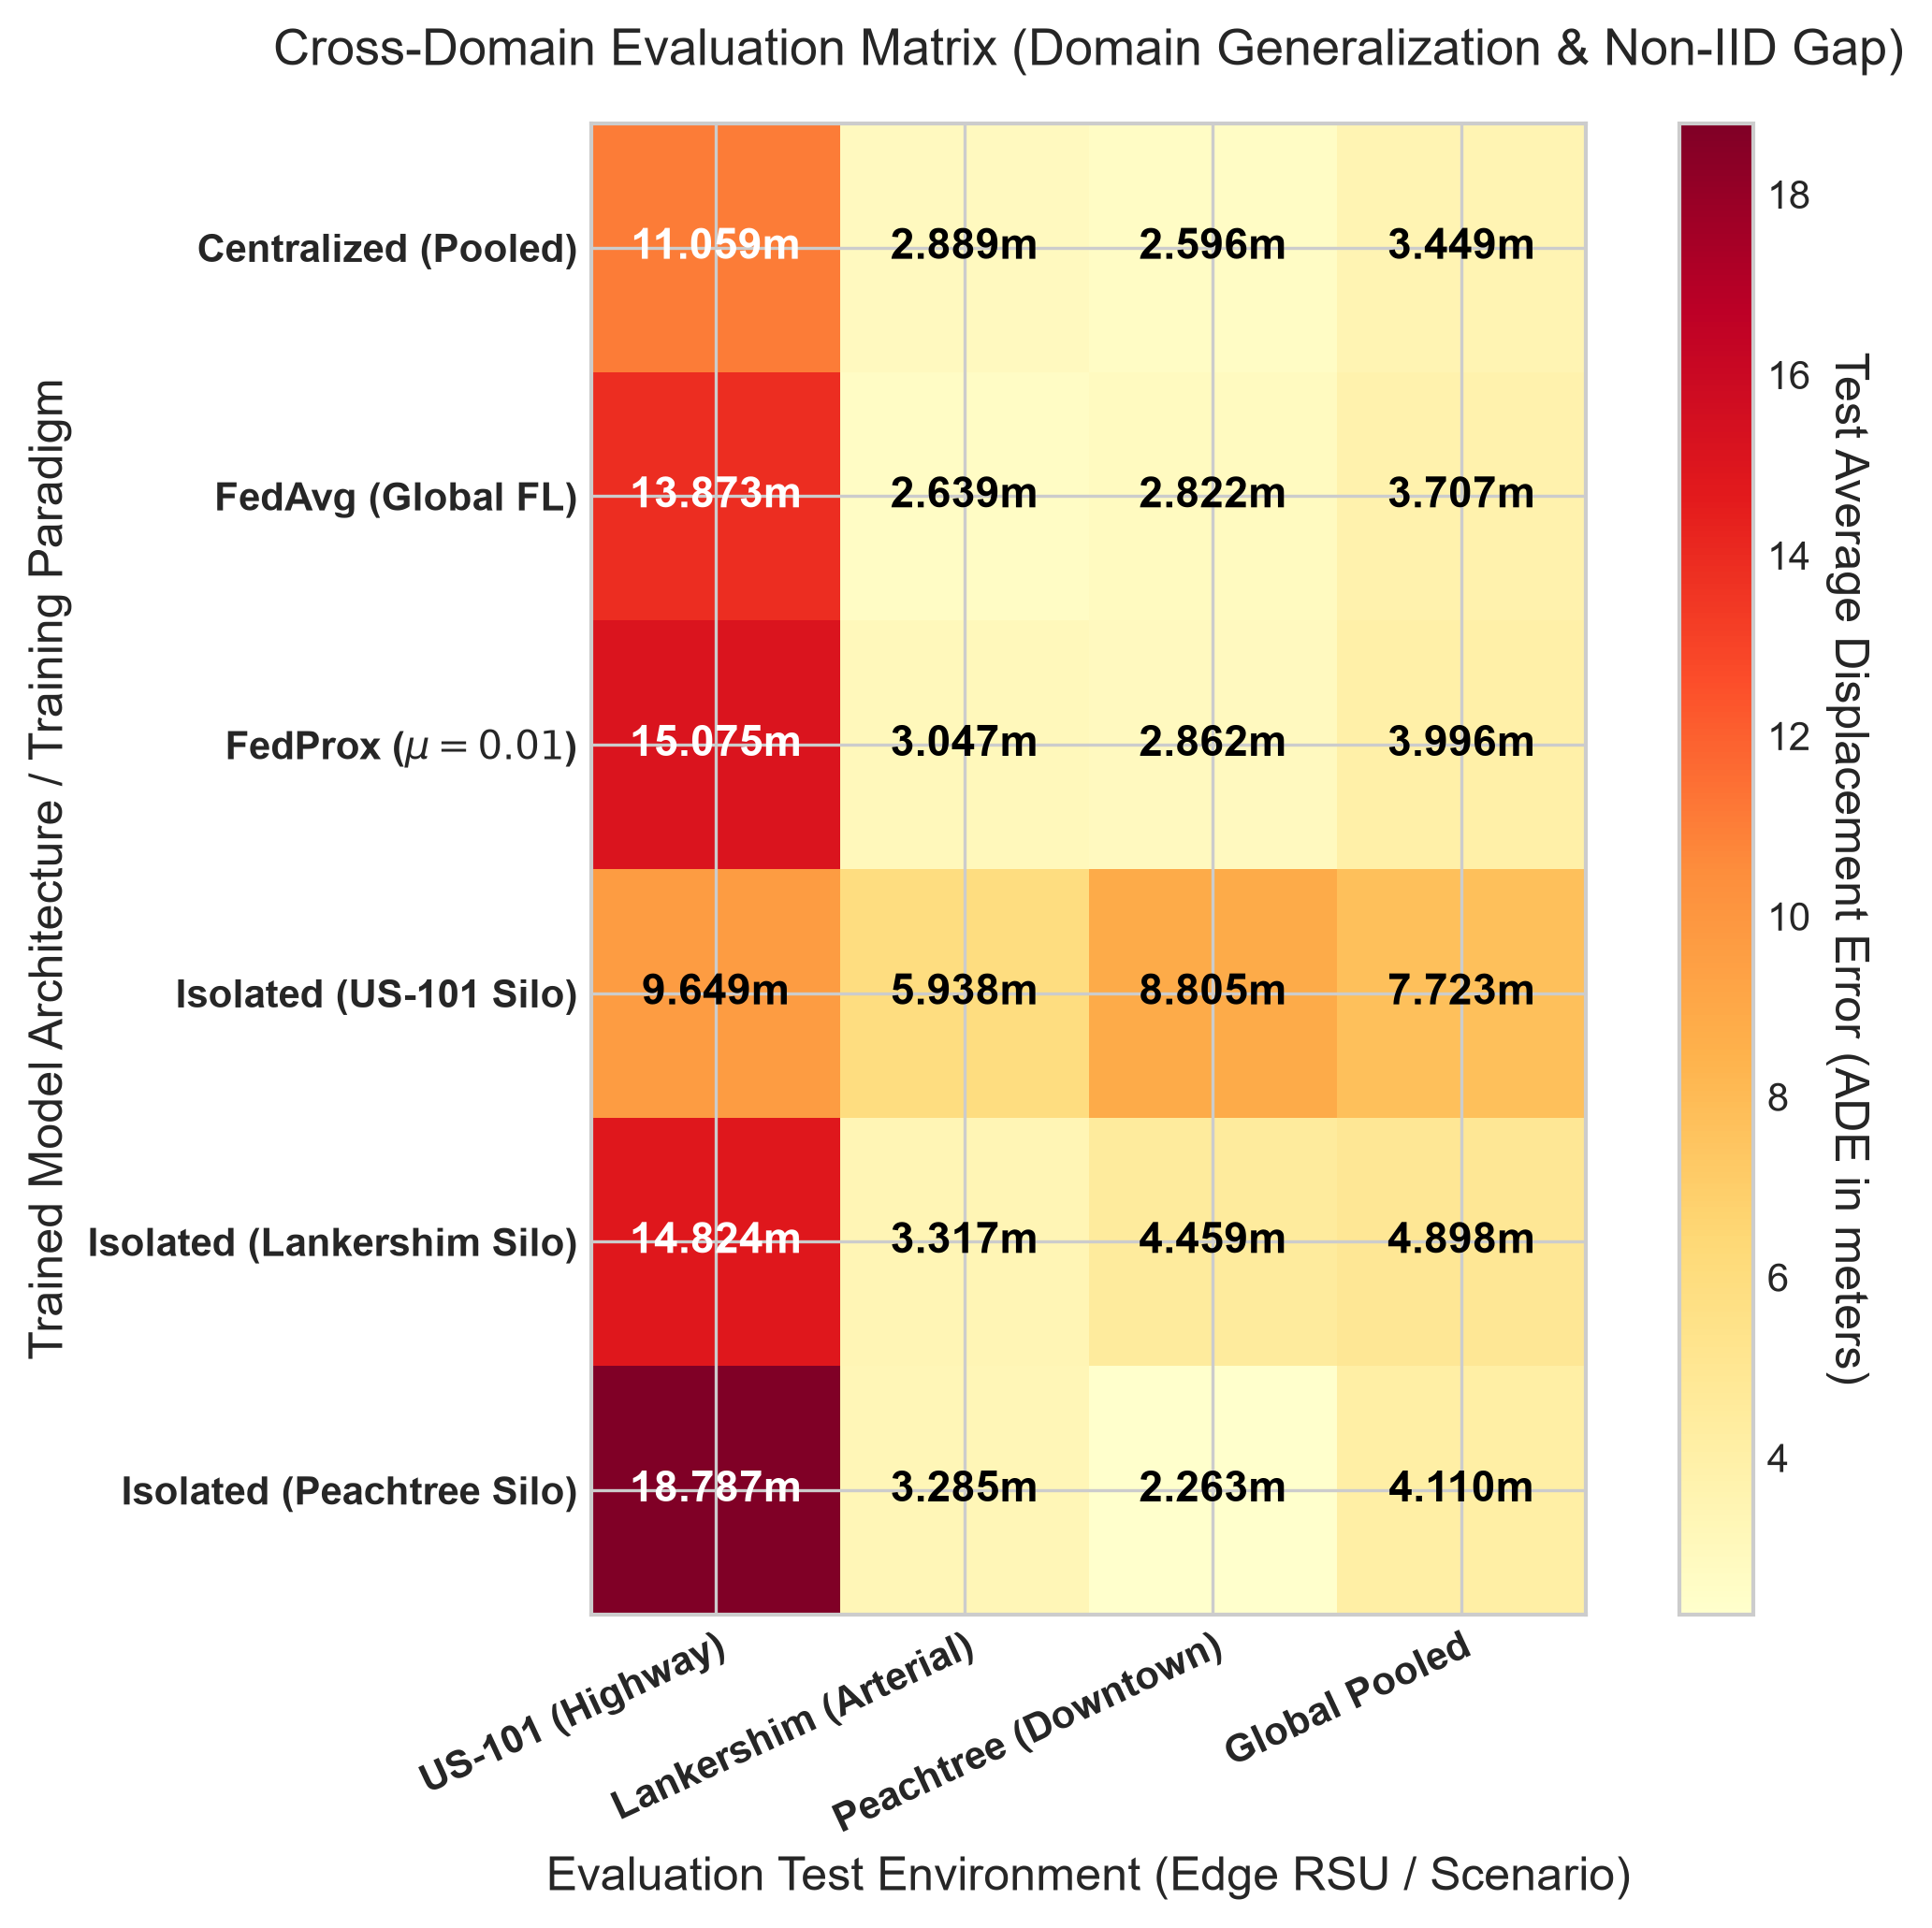
\includegraphics[width=\columnwidth]{fig4_cross_domain_generalization.png}
\caption{Cross-domain evaluation heatmap illustrating out-of-distribution domain collapse for isolated silo models compared to federated baselines.}
\label{fig:cross_domain}
\end{figure}

\begin{figure}[!t]
\centering
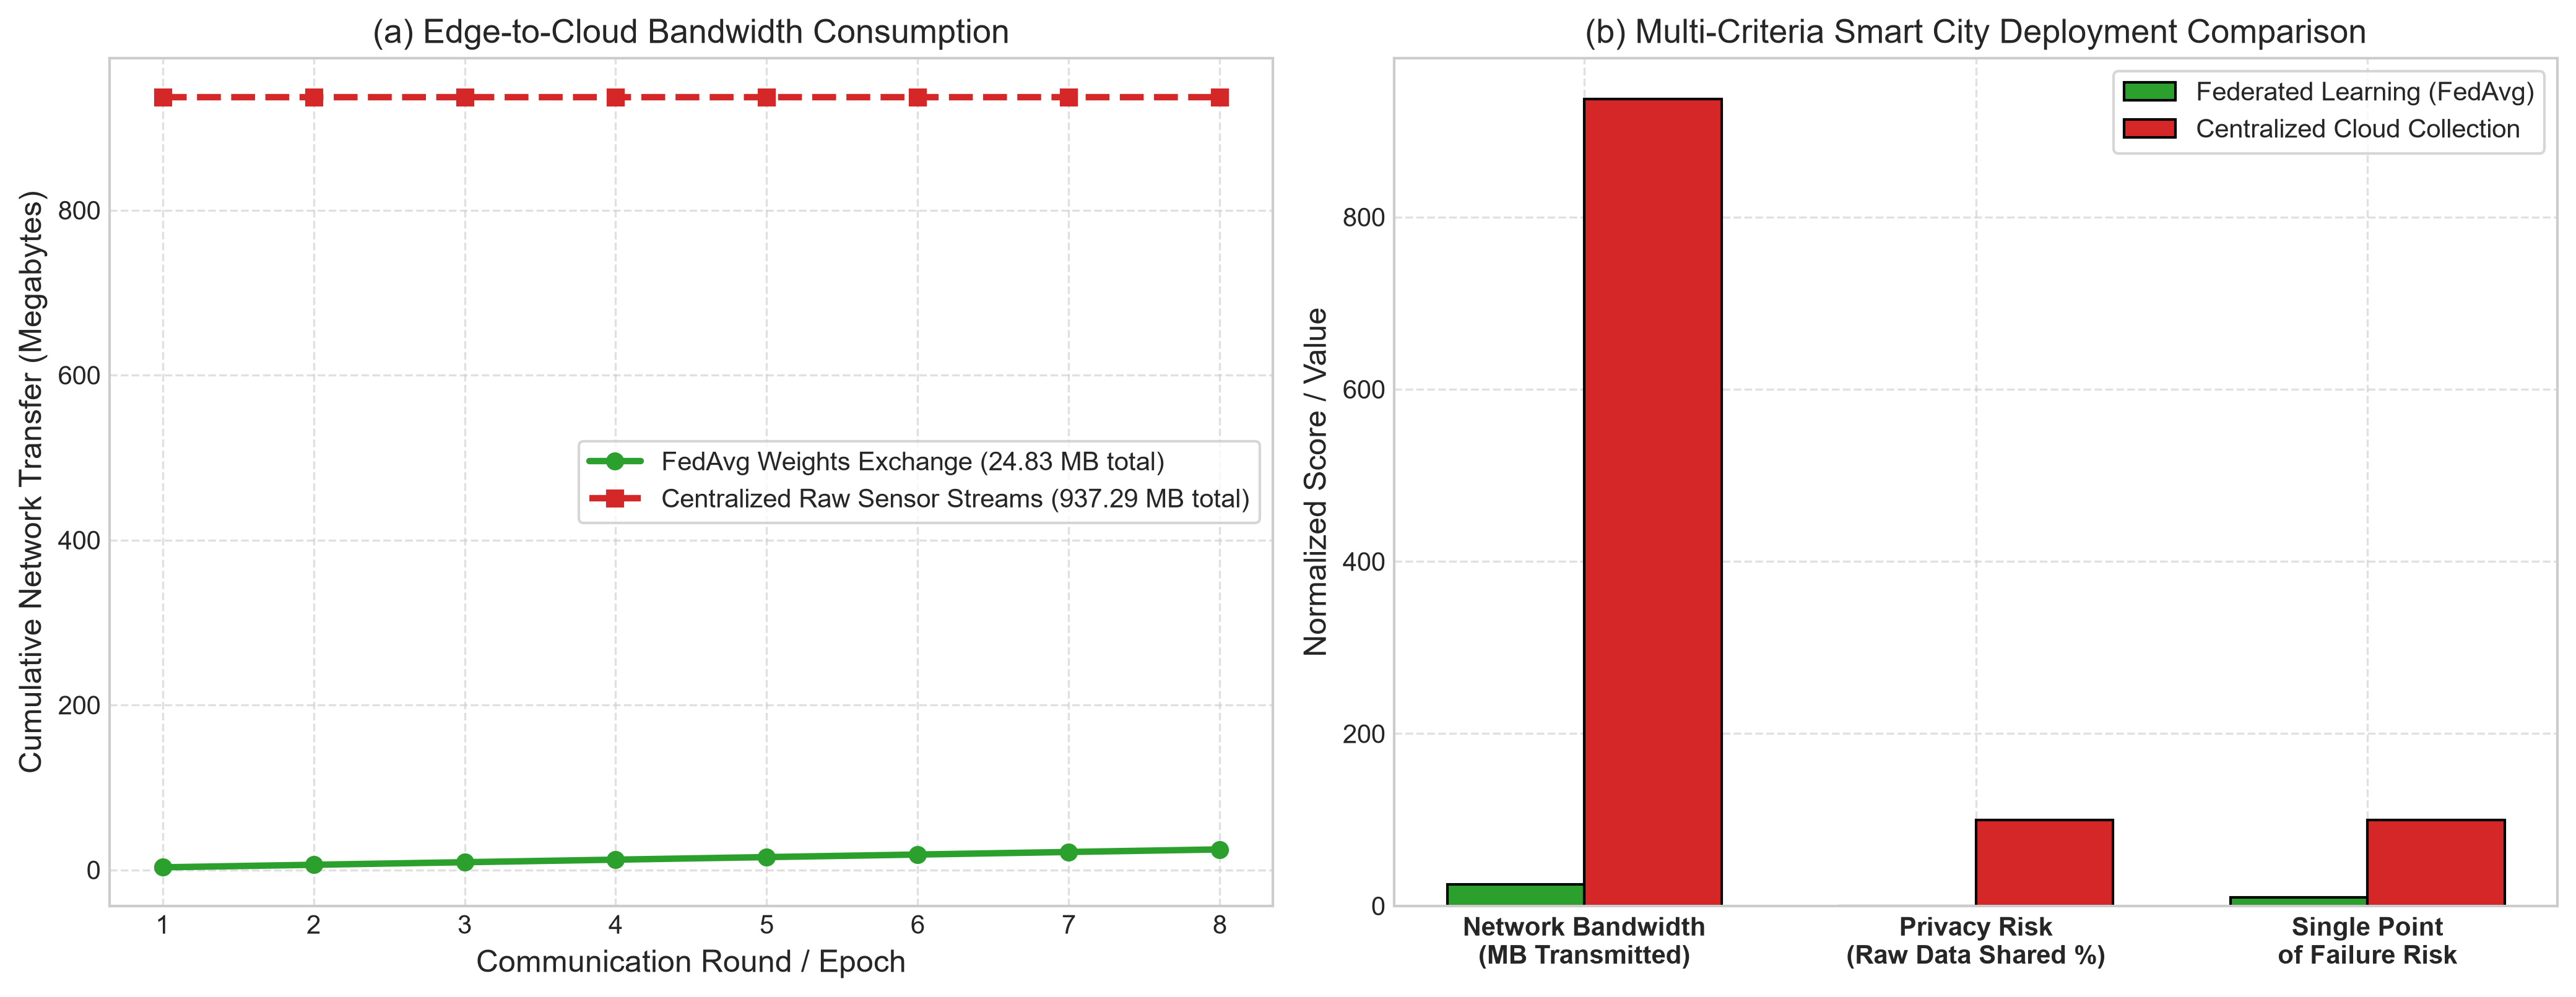
\includegraphics[width=\columnwidth]{fig5_communication_privacy_tradeoff.png}
\caption{Wireless communication efficiency: cumulative edge-to-cloud backhaul network bandwidth consumption across training rounds.}
\label{fig:comm_tradeoff}
\end{figure}

\begin{figure}[!t]
\centering
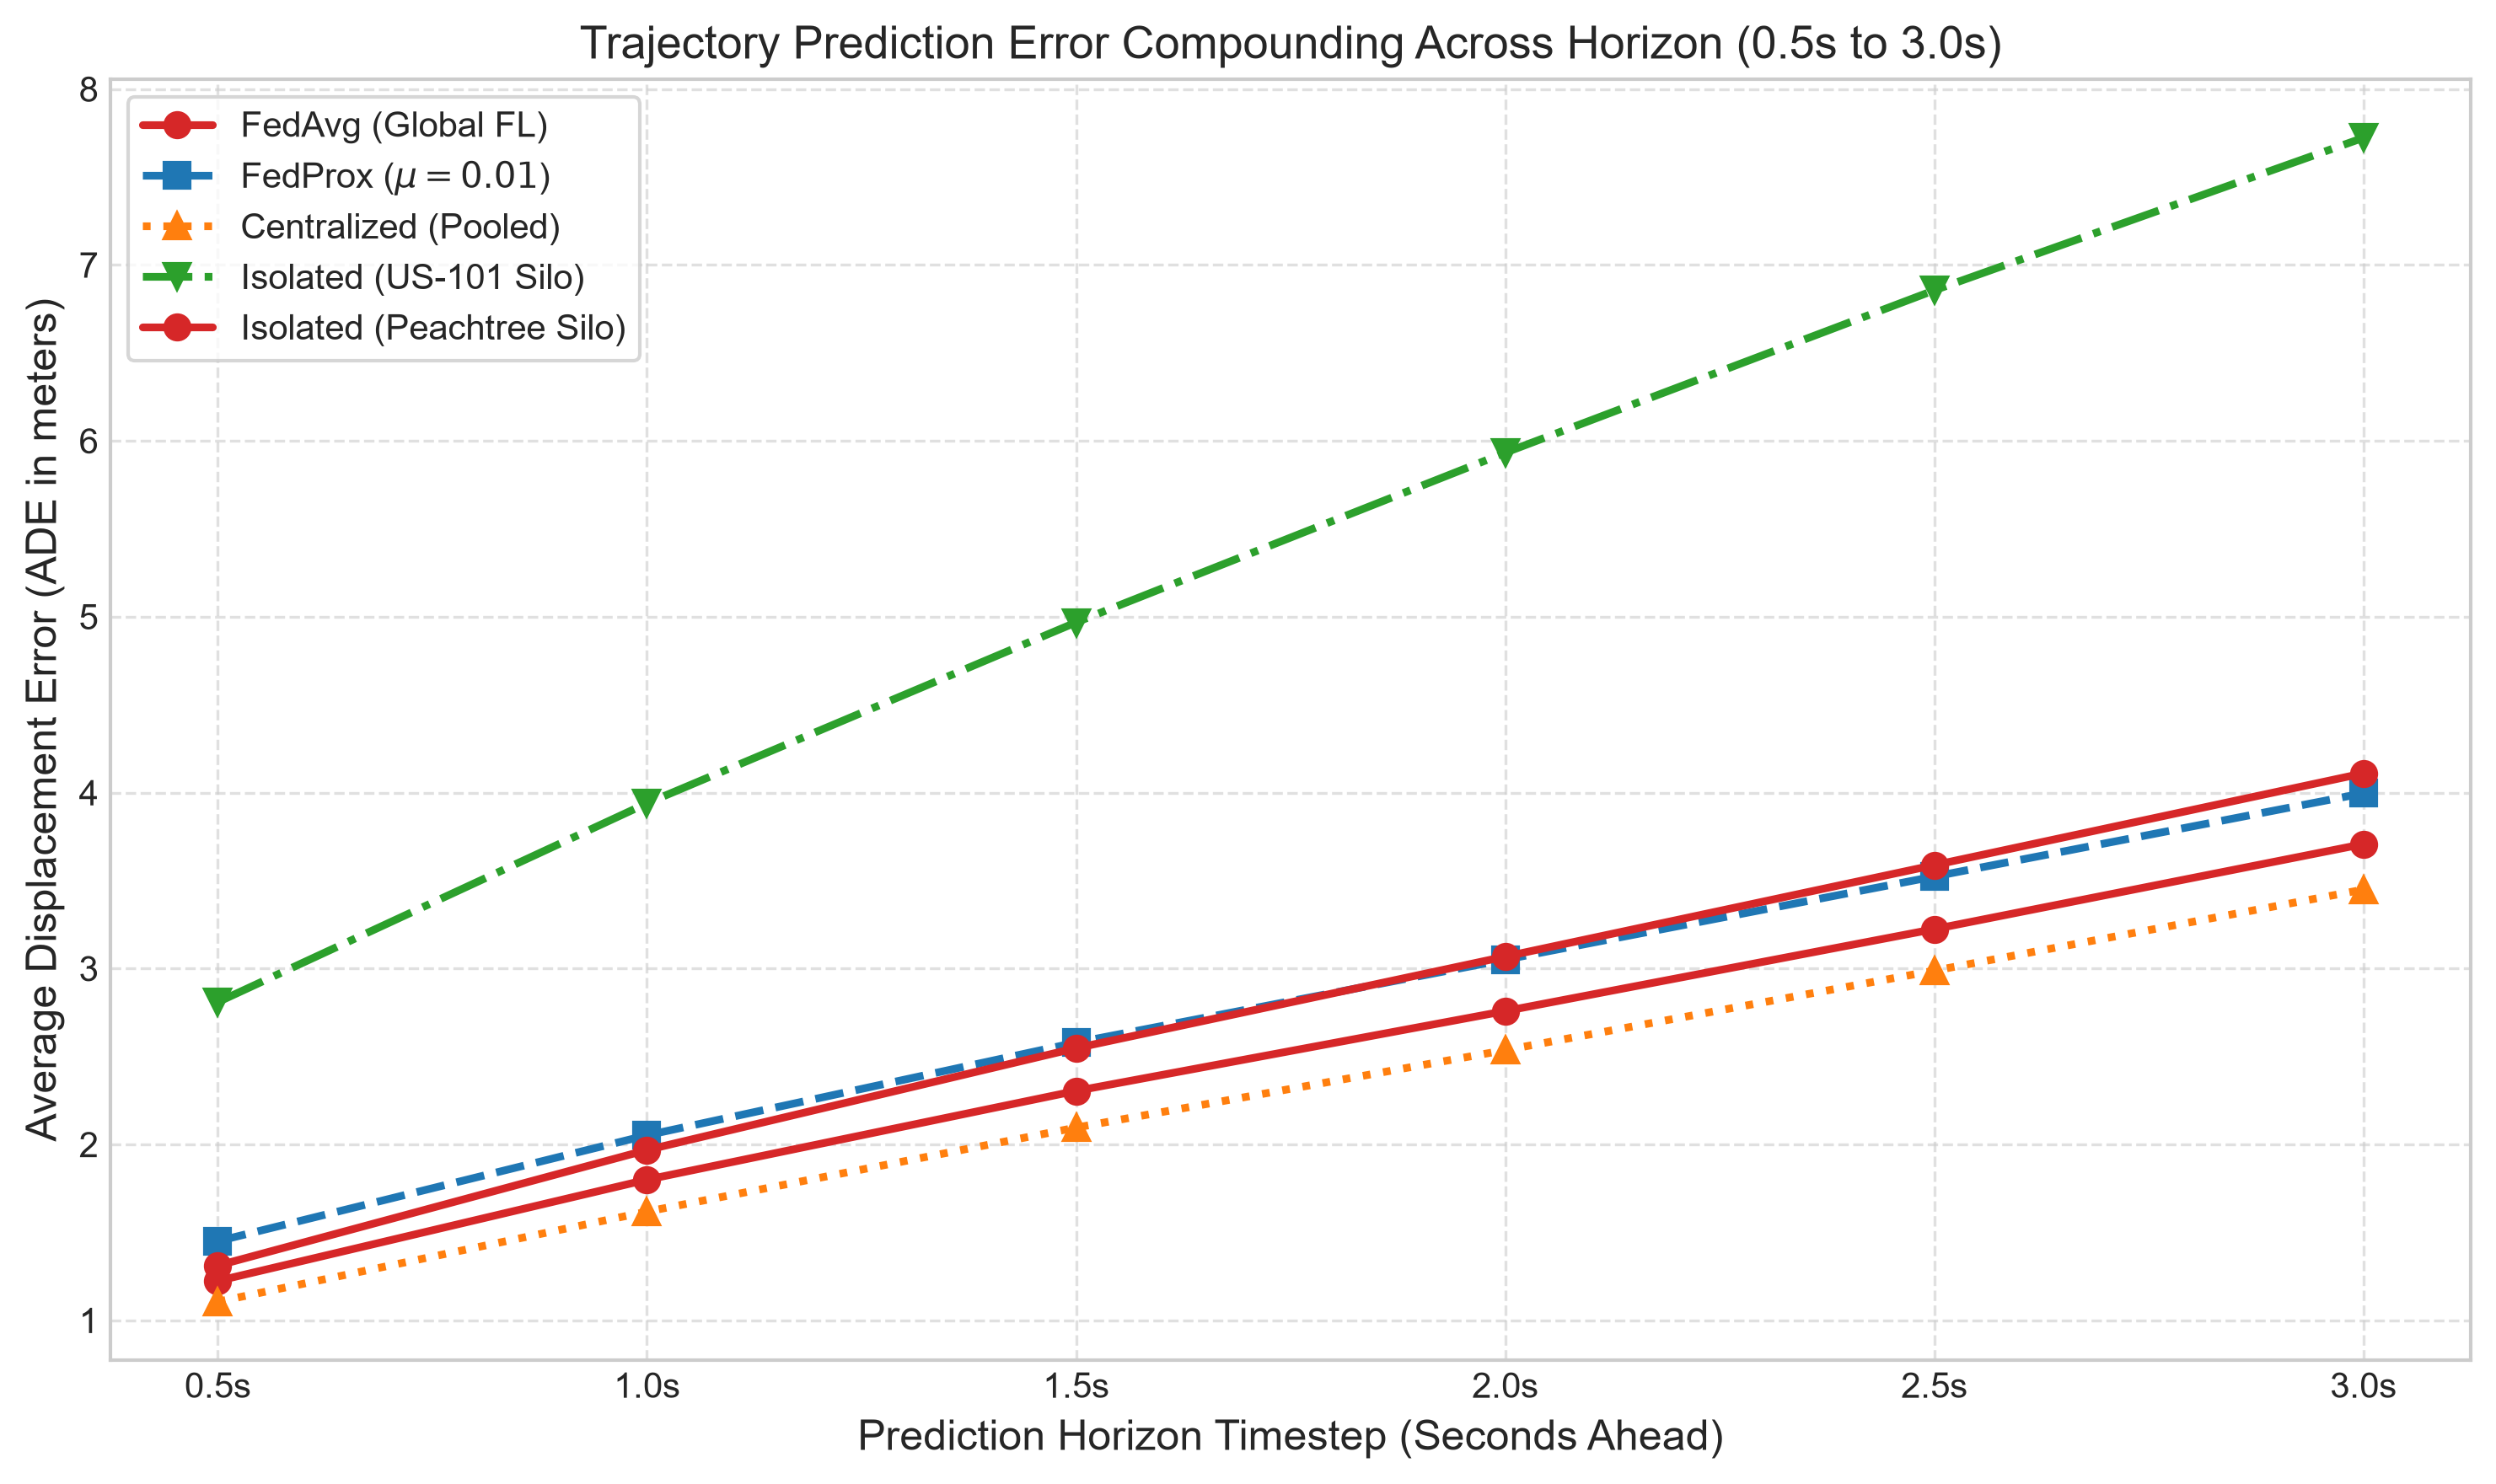
\includegraphics[width=\columnwidth]{fig6_horizon_error_growth.png}
\caption{Multi-horizon ADE error progression curves across forecast horizons from $0.5$\,s to $3.0$\,s.}
\label{fig:horizon_growth}
\end{figure}

In terms of global displacement error, FedPer achieved a Global Pooled ADE of $2.951$\,m and an FDE of $4.835$\,m. This performance improves upon centralized pooled training ($3.142$\,m ADE, $5.101$\,m FDE) by $6.1\%$. FedPer also outperforms canonical FedAvg ($3.656$\,m ADE) by $19.3\%$ and FedProx ($3.710$\,m ADE) by $20.5\%$. Across individual zones, FedPer achieved an ADE of $9.917$\,m on the US-101 freeway, $2.859$\,m on Lankershim Boulevard, and $1.837$\,m on Peachtree Street.

Models trained in isolated silos suffered severe performance degradation when tested outside their home domains (Fig.~\ref{fig:cross_domain}). For example, the Peachtree silo model scored $1.757$\,m ADE locally, but its error surged to $18.380$\,m ADE on US-101 highway traffic, representing a $10.46$-fold error increase. Similarly, the US-101 silo model achieved $9.253$\,m ADE on highway test data, but degraded to $7.778$\,m ADE on Peachtree downtown, which is $4.23$ times higher than FedPer. In network communication, centralized training required transmitting $937.29$\,MB of raw coordinate files. In contrast, FedAvg transferred $37.24$\,MB, while FedPer transmitted $36.65$\,MB. FedPer reduced backhaul data transfer by $96.08\%$ relative to raw coordinate streaming.

\subsection{Controlled Heterogeneity Resilience}
\label{sec:heterogeneity_resilience}
Table~\ref{tab:controlled_hetero} and Fig.~\ref{fig:hetero_personalization} report algorithmic performance under controlled synthetic non-IID regimes: Low ($\overline{\mathrm{JSD}} = 0.0524$), Medium ($\overline{\mathrm{JSD}} = 0.1088$), and High ($\overline{\mathrm{JSD}} = 0.1335$).

\begin{table}[!t]
\caption{Algorithmic Performance Under Controlled Synthetic Geographic Non-IID Regimes}
\label{tab:controlled_hetero}
\centering
\resizebox{\columnwidth}{!}{%
\begin{tabular}{lccccc}
\toprule
\textbf{Heterogeneity Level} & \textbf{FedAvg (m)} & \textbf{FedPer (m)} & \textbf{pFedMe (m)} & \textbf{FedPer Adv.} & \textbf{pFedMe Adv.} \\
\midrule
Low ($\overline{\mathrm{JSD}}=0.0524$) & 6.315 & 5.033 & 9.101 & +1.282\,m & -2.786\,m \\
Medium ($\overline{\mathrm{JSD}}=0.1088$) & 6.803 & 5.038 & 8.859 & +1.765\,m & -2.056\,m \\
High ($\overline{\mathrm{JSD}}=0.1335$) & 7.074 & 5.898 & 8.571 & +1.176\,m & -1.497\,m \\
\bottomrule
\end{tabular}%
}
\end{table}

\begin{figure}[!t]
\centering
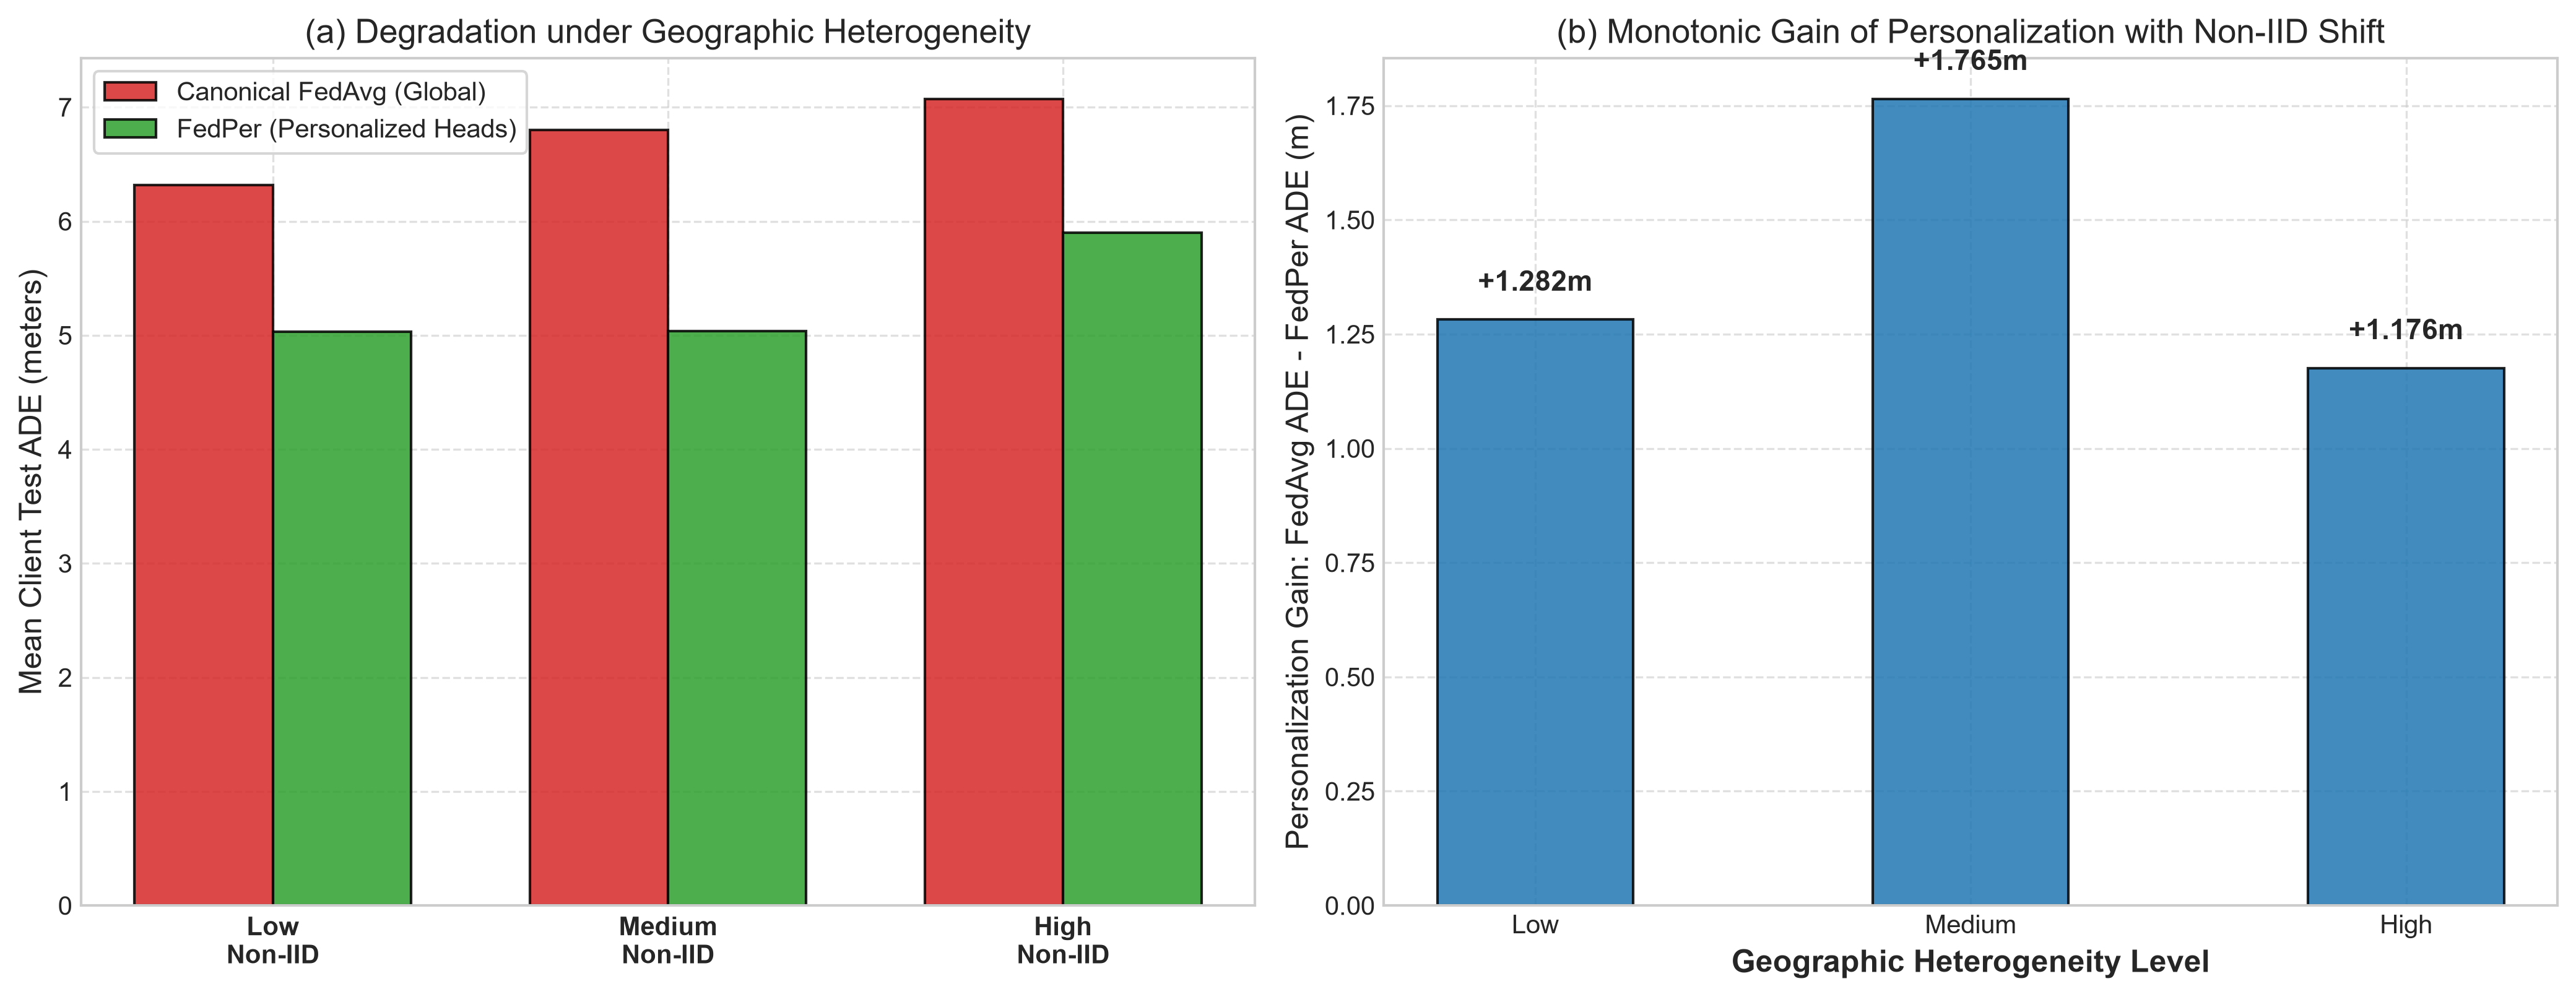
\includegraphics[width=\columnwidth]{fig7_heterogeneity_vs_personalization.png}
\caption{Controlled heterogeneity resilience: FedAvg degrades from $6.315$\,m to $7.074$\,m as non-IID shift escalates, whereas FedPer maintains localized domain specialization.}
\label{fig:hetero_personalization}
\end{figure}

As data heterogeneity increased from Low ($0.0524$) to High ($0.1335$), standard FedAvg exhibited continuous error inflation. Its mean zone ADE increased from $6.315$\,m to $7.074$\,m, reflecting a $0.759$\,m error degradation. In contrast, FedPer maintained strong localized adaptation across all three regimes. FedPer outperformed FedAvg by $1.282$\,m under Low heterogeneity, by $1.765$\,m under Medium heterogeneity, and by $1.176$\,m under High heterogeneity.

\subsection{Privacy Attack Auditing and Spatial Fairness}
\label{sec:privacy_fairness}
Table~\ref{tab:privacy_dlg} and Fig.~\ref{fig:privacy_reconstruction} report privacy audit results under DLG gradient inversion attacks and Gaussian DP defenses. Table~\ref{tab:fairness} and Fig.~\ref{fig:fairness_comp} detail spatial fairness and disparity metrics. Table~\ref{tab:pareto} and Fig.~\ref{fig:pareto_frontier} summarize trade-offs across accuracy, bandwidth, fairness, and differential privacy.

\begin{table*}[!t]
\caption{Privacy Auditing Results: Deep Leakage from Gradients (DLG) and Gaussian Differential Privacy Defense Bounds}
\label{tab:privacy_dlg}
\centering
\resizebox{\textwidth}{!}{%
\begin{tabular}{llcccccc}
\toprule
\textbf{FL Method} & \textbf{Defense Mechanism} & \textbf{Noise ($\sigma$)} & \textbf{Budget ($\epsilon$)} & \textbf{Recon. Error (m)} & \textbf{Cosine Sim.} & \textbf{Input MSE} & \textbf{Target MSE} \\
\midrule
FedAvg & None (Unprotected Gradients) & 0.0 & $\infty$ & 1.0858 & 0.5513 & 1.3248 & 1.5297 \\
FedAvg & Gaussian DP & 0.5 & 9.69 & 6.4579 & 0.1942 & 24.7421 & 5.9887 \\
FedAvg & Gaussian DP & 1.0 & 4.84 & 7.7608 & -0.0453 & 32.2346 & 11.5636 \\
FedAvg & Gaussian DP & 2.0 & 2.42 & 8.0940 & 0.0251 & 32.7436 & 14.2970 \\
\midrule
\textbf{FedPer} & \textbf{Head Isolation} & \textbf{0.0} & \textbf{$\infty$} & \textbf{1.3058} & \textbf{0.6342} & \textbf{1.6010} & \textbf{1.5854} \\
FedPer & Head Isolation + DP & 0.5 & 9.69 & 8.6907 & -0.0014 & 40.4046 & 44.1721 \\
FedPer & Head Isolation + DP & 1.0 & 4.84 & 8.1955 & 0.0545 & 38.6335 & 57.7735 \\
FedPer & Head Isolation + DP & 2.0 & 2.42 & 8.5839 & -0.1062 & 44.9978 & 69.6027 \\
\bottomrule
\end{tabular}%
}
\end{table*}

\begin{figure}[!t]
\centering
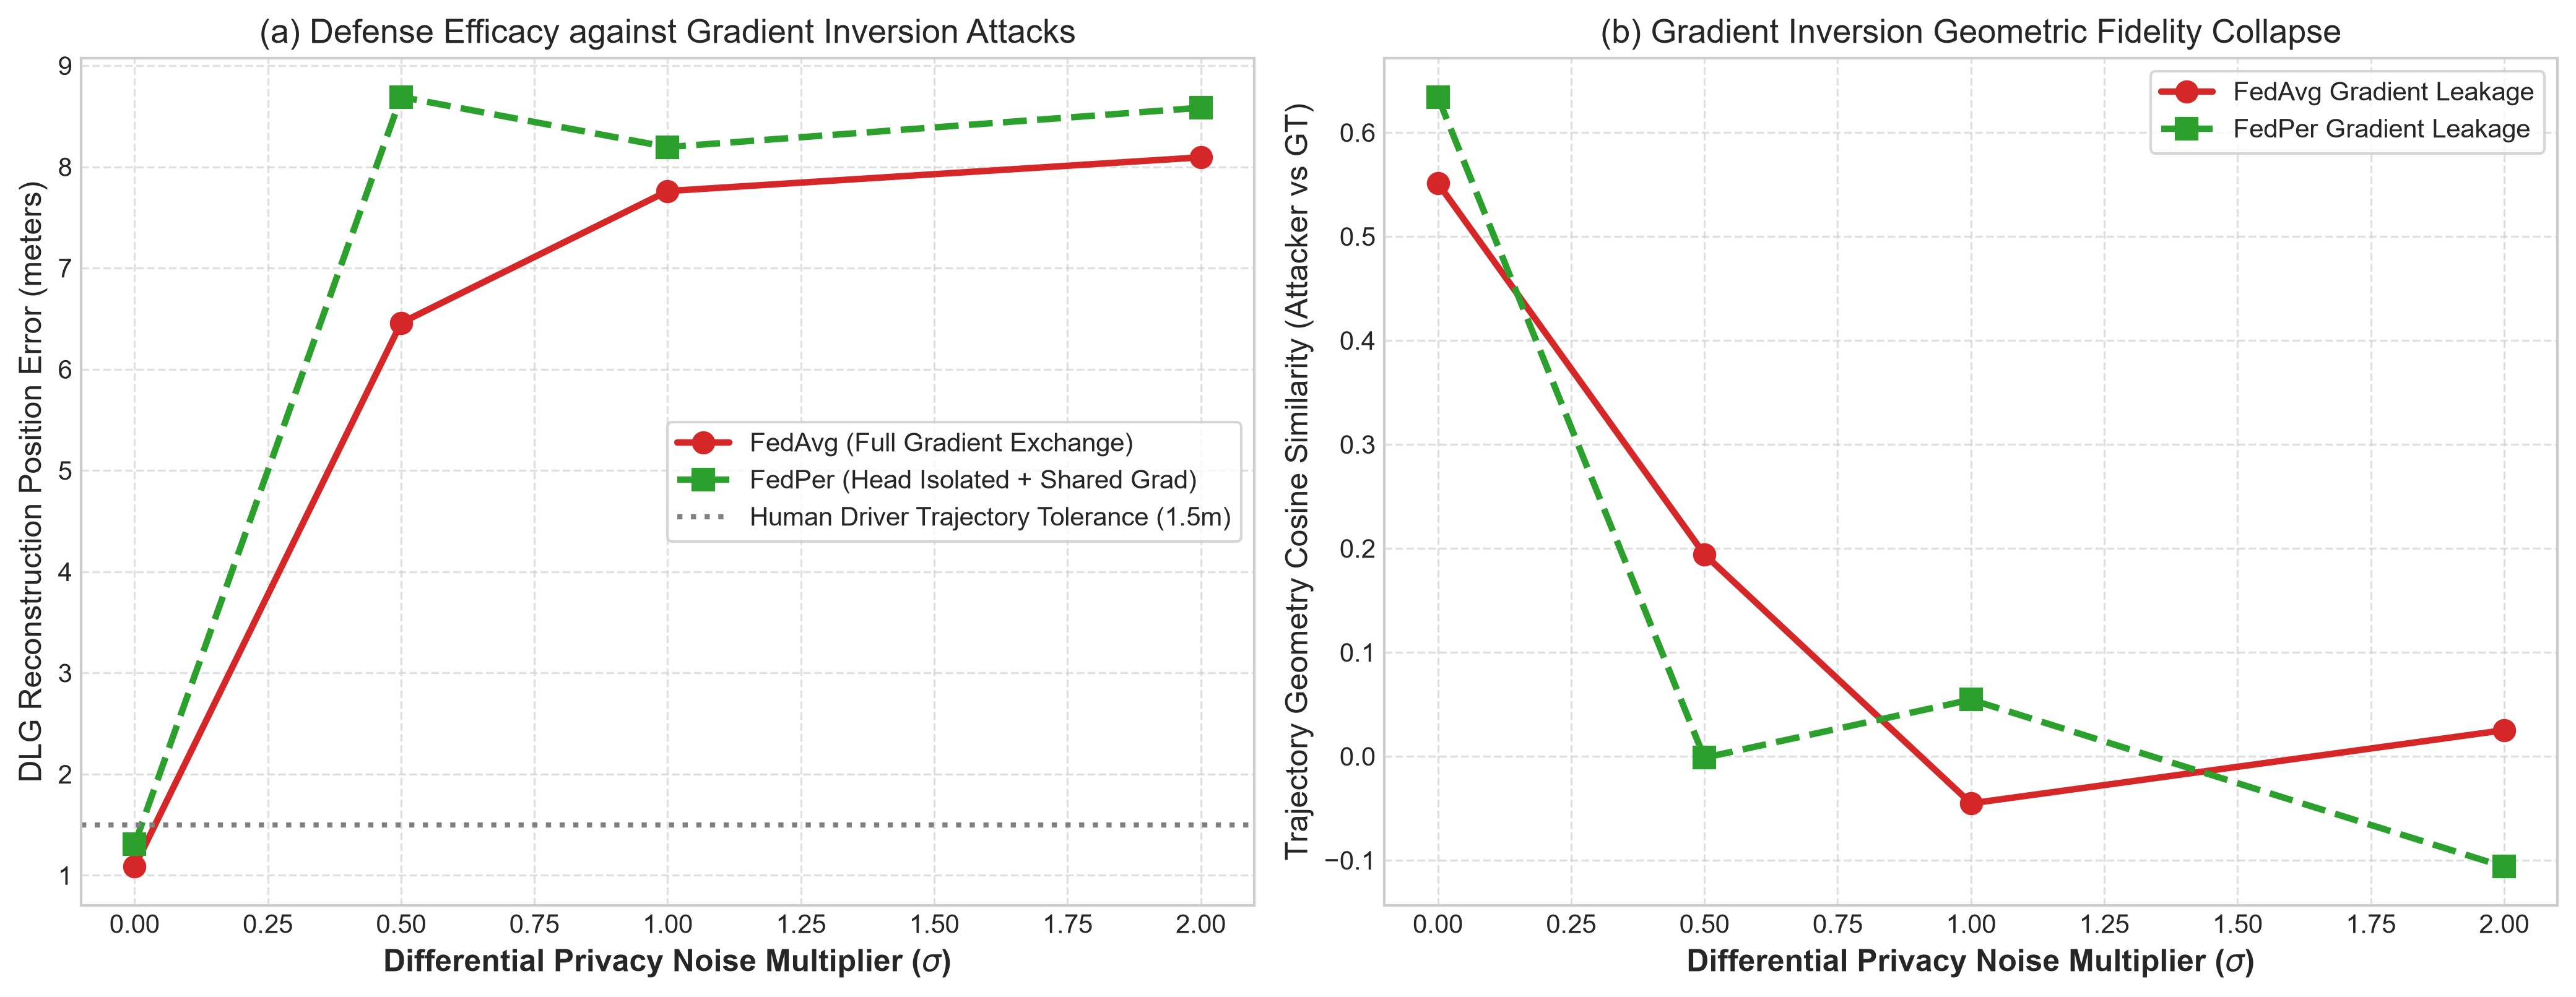
\includegraphics[width=\columnwidth]{fig8_privacy_reconstruction_vs_dp.png}
\caption{Trajectory reconstruction error under DLG gradient inversion attacks as a function of Gaussian DP noise multiplier $\sigma$.}
\label{fig:privacy_reconstruction}
\end{figure}

Under unprotected FedAvg exchanges, the DLG attack reconstructed vehicle trajectory paths with an average error of $1.0858$\,m and a cosine similarity of $0.5513$. Injecting Gaussian DP noise at $\sigma = 0.5$ ($\epsilon = 9.69$) degraded gradient matching, increasing reconstruction error to $6.4579$\,m. Raising noise to $\sigma = 1.0$ ($\epsilon = 4.84$) pushed reconstruction error to $7.7608$\,m and reduced cosine similarity to $-0.0453$. Under FedPer, withholding the regression head prevented an adversary from matching output gradients. Adding Gaussian DP ($\sigma = 0.5$) to FedPer raised the reconstruction error to $8.6907$\,m and target MSE to $44.1721$. In membership inference audits, shadow models achieved an AUC of $0.4994$ ($52.75\%$ accuracy) on FedAvg and $0.4713$ ($51.00\%$ accuracy) on FedPer, confirming baseline chance-level privacy protection.

\begin{table*}[!t]
\caption{Personalization, Spatial Disparity, and Algorithmic Fairness Analysis Across Evaluated Paradigms}
\label{tab:fairness}
\centering
\resizebox{\textwidth}{!}{%
\begin{tabular}{lcccccccc}
\toprule
\textbf{Model Architecture} & \textbf{Global ADE (m)} & \textbf{Mean Zone ADE} & \textbf{Worst-Zone ADE} & \textbf{Best-Zone ADE} & \textbf{Disparity Gap} & \textbf{Fairness CoV} & \textbf{PFL Recovery} & \textbf{Comm (MB)} \\
\midrule
Centralized (Pooled) & 3.142 & 4.892 & 9.576 & 2.391 & 7.185 & 67.77\% & 100.0\% & 937.29 \\
FedAvg (Global FL) & 3.656 & 6.587 & 14.539 & 2.529 & 12.010 & 85.36\% & 0.0\% & 37.24 \\
FedProx ($\mu=0.01$) & 3.710 & 6.673 & 14.656 & 2.578 & 12.078 & 84.59\% & 0.0\% & 37.24 \\
\textbf{FedPer (Personalized)} & \textbf{2.951} & \textbf{4.871} & \textbf{9.917} & \textbf{1.837} & \textbf{8.081} & \textbf{73.75\%} & \textbf{100.0\%} & \textbf{36.65} \\
pFedMe (Moreau) & 5.981 & 8.440 & 15.213 & 4.623 & 10.590 & 56.90\% & 0.0\% & 37.24 \\
Isolated (US-101 Silo) & 6.785 & 7.343 & 9.253 & 4.999 & 4.254 & 24.02\% & 0.0\% & 0.00 \\
Isolated (Lankershim) & 4.266 & 7.115 & 14.966 & 2.691 & 12.275 & 78.22\% & 0.0\% & 0.00 \\
Isolated (Peachtree) & 3.596 & 7.625 & 18.380 & 1.757 & 16.623 & 99.88\% & 0.0\% & 0.00 \\
\bottomrule
\end{tabular}%
}
\end{table*}

\begin{figure}[!t]
\centering
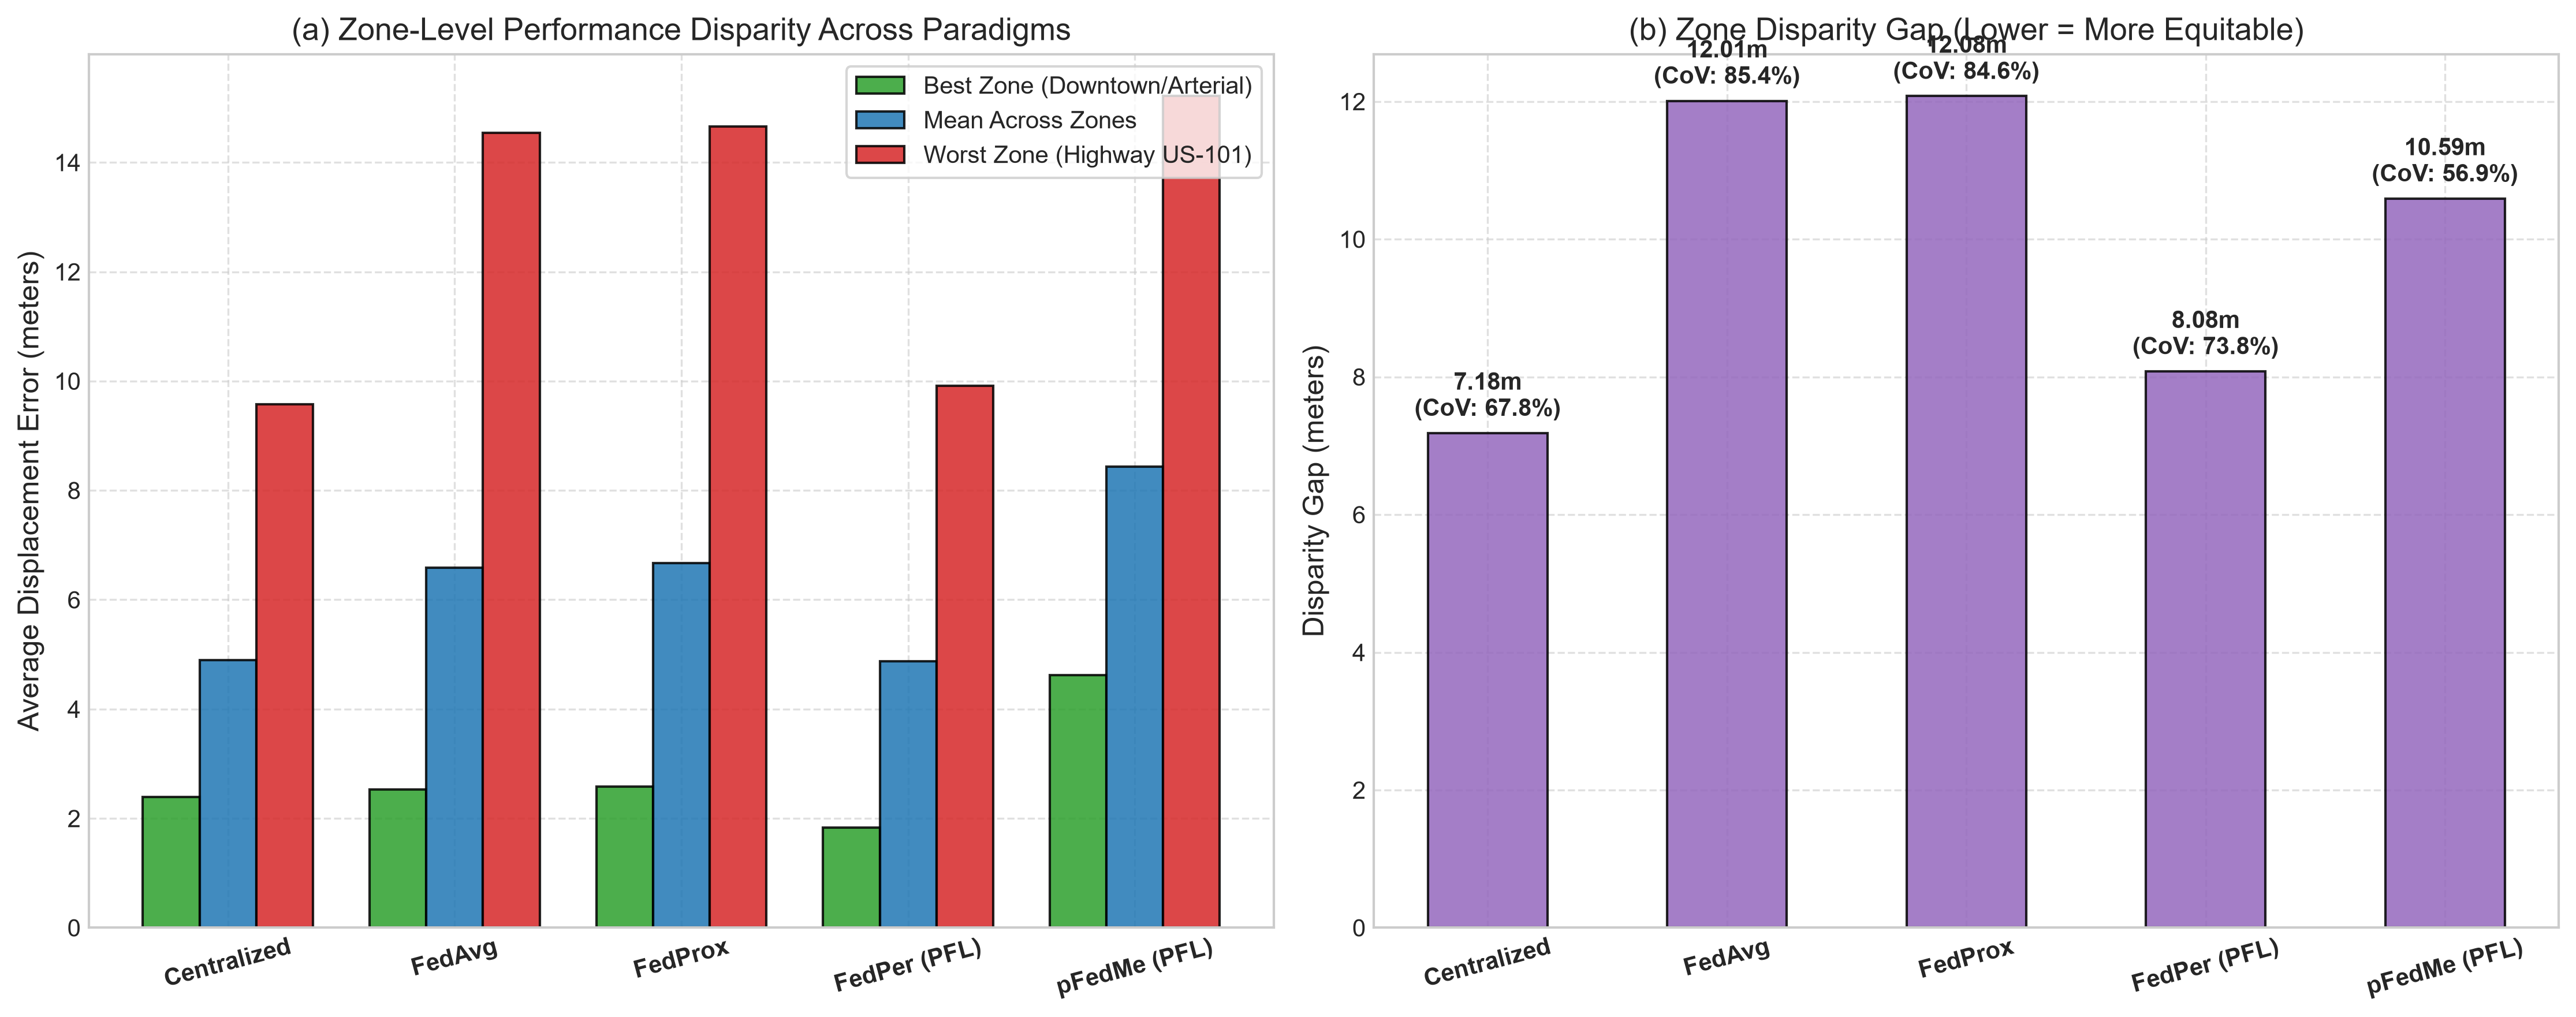
\includegraphics[width=\columnwidth]{fig9_fairness_disparity_comparison.png}
\caption{Algorithmic fairness and regional disparity gap comparison: FedPer compresses the spatial disparity gap from $12.010$\,m to $8.081$\,m while lowering CoV from $85.36\%$ to $73.75\%$.}
\label{fig:fairness_comp}
\end{figure}

In spatial fairness evaluation (Table~\ref{tab:fairness} and Fig.~\ref{fig:fairness_comp}), standard FedAvg produced an ADE of $14.539$\,m on the US-101 freeway and $2.529$\,m on Lankershim Boulevard. This contrast created an inter-zone disparity gap of $12.010$\,m and a Coefficient of Variation (CoV) of $85.36\%$. FedPer reduced the US-101 error to $9.917$\,m, representing a $31.79\%$ error reduction, while improving Peachtree error to $1.837$\,m, a $27.36\%$ gain. These improvements narrowed the zone disparity gap to $8.081$\,m, cutting inter-zone disparity by $32.71\%$ and reducing the fairness CoV to $73.75\%$.

\begin{table*}[!t]
\caption{Integrated Accuracy--Communication--Fairness--Privacy Pareto Optimization Matrix}
\label{tab:pareto}
\centering
\resizebox{\textwidth}{!}{%
\begin{tabular}{lcccccccc}
\toprule
\textbf{Model Configuration} & \textbf{Global ADE (m)} & \textbf{Worst ADE (m)} & \textbf{Fairness CoV} & \textbf{Comm (MB)} & \textbf{DLG Error (m)} & \textbf{Cosine Sim.} & \textbf{MIA AUC} & \textbf{Privacy Budget ($\epsilon$)} \\
\midrule
Centralized (Pooled) & 3.142 & 9.576 & 67.77\% & 937.29 & 999.00 & 0.000 & 0.4994 & N/A (No Grad Sharing) \\
FedAvg (Global FL) & 3.656 & 14.539 & 85.36\% & 37.24 & 1.086 & 0.551 & 0.4994 & $\infty$ \\
FedProx ($\mu=0.01$) & 3.710 & 14.656 & 84.59\% & 37.24 & 1.086 & 0.551 & 0.4994 & $\infty$ \\
\textbf{FedPer (Personalized)} & \textbf{2.951} & \textbf{9.917} & \textbf{73.75\%} & \textbf{36.65} & \textbf{1.306} & \textbf{0.634} & \textbf{0.4713} & \textbf{$\infty$ (Head Private)} \\
pFedMe (Moreau) & 5.981 & 15.213 & 56.90\% & 37.24 & 1.086 & 0.551 & 0.4994 & $\infty$ \\
Isolated (US-101 Silo) & 6.785 & 9.253 & 24.02\% & 0.00 & 999.00 & 0.000 & 0.4994 & N/A (No Grad Sharing) \\
Isolated (Lankershim) & 4.266 & 14.966 & 78.22\% & 0.00 & 999.00 & 0.000 & 0.4994 & N/A (No Grad Sharing) \\
Isolated (Peachtree) & 3.596 & 18.380 & 99.88\% & 0.00 & 999.00 & 0.000 & 0.4994 & N/A (No Grad Sharing) \\
DP-FedAvg ($\sigma=0.5$) & 3.948 & 15.848 & 89.63\% & 37.24 & 6.458 & 0.194 & 0.4240 & 9.69 \\
DP-FedAvg ($\sigma=1.0$) & 4.314 & 17.447 & 93.90\% & 37.24 & 7.761 & -0.045 & 0.3600 & 4.84 \\
\bottomrule
\end{tabular}%
}
\end{table*}

\begin{figure}[!t]
\centering
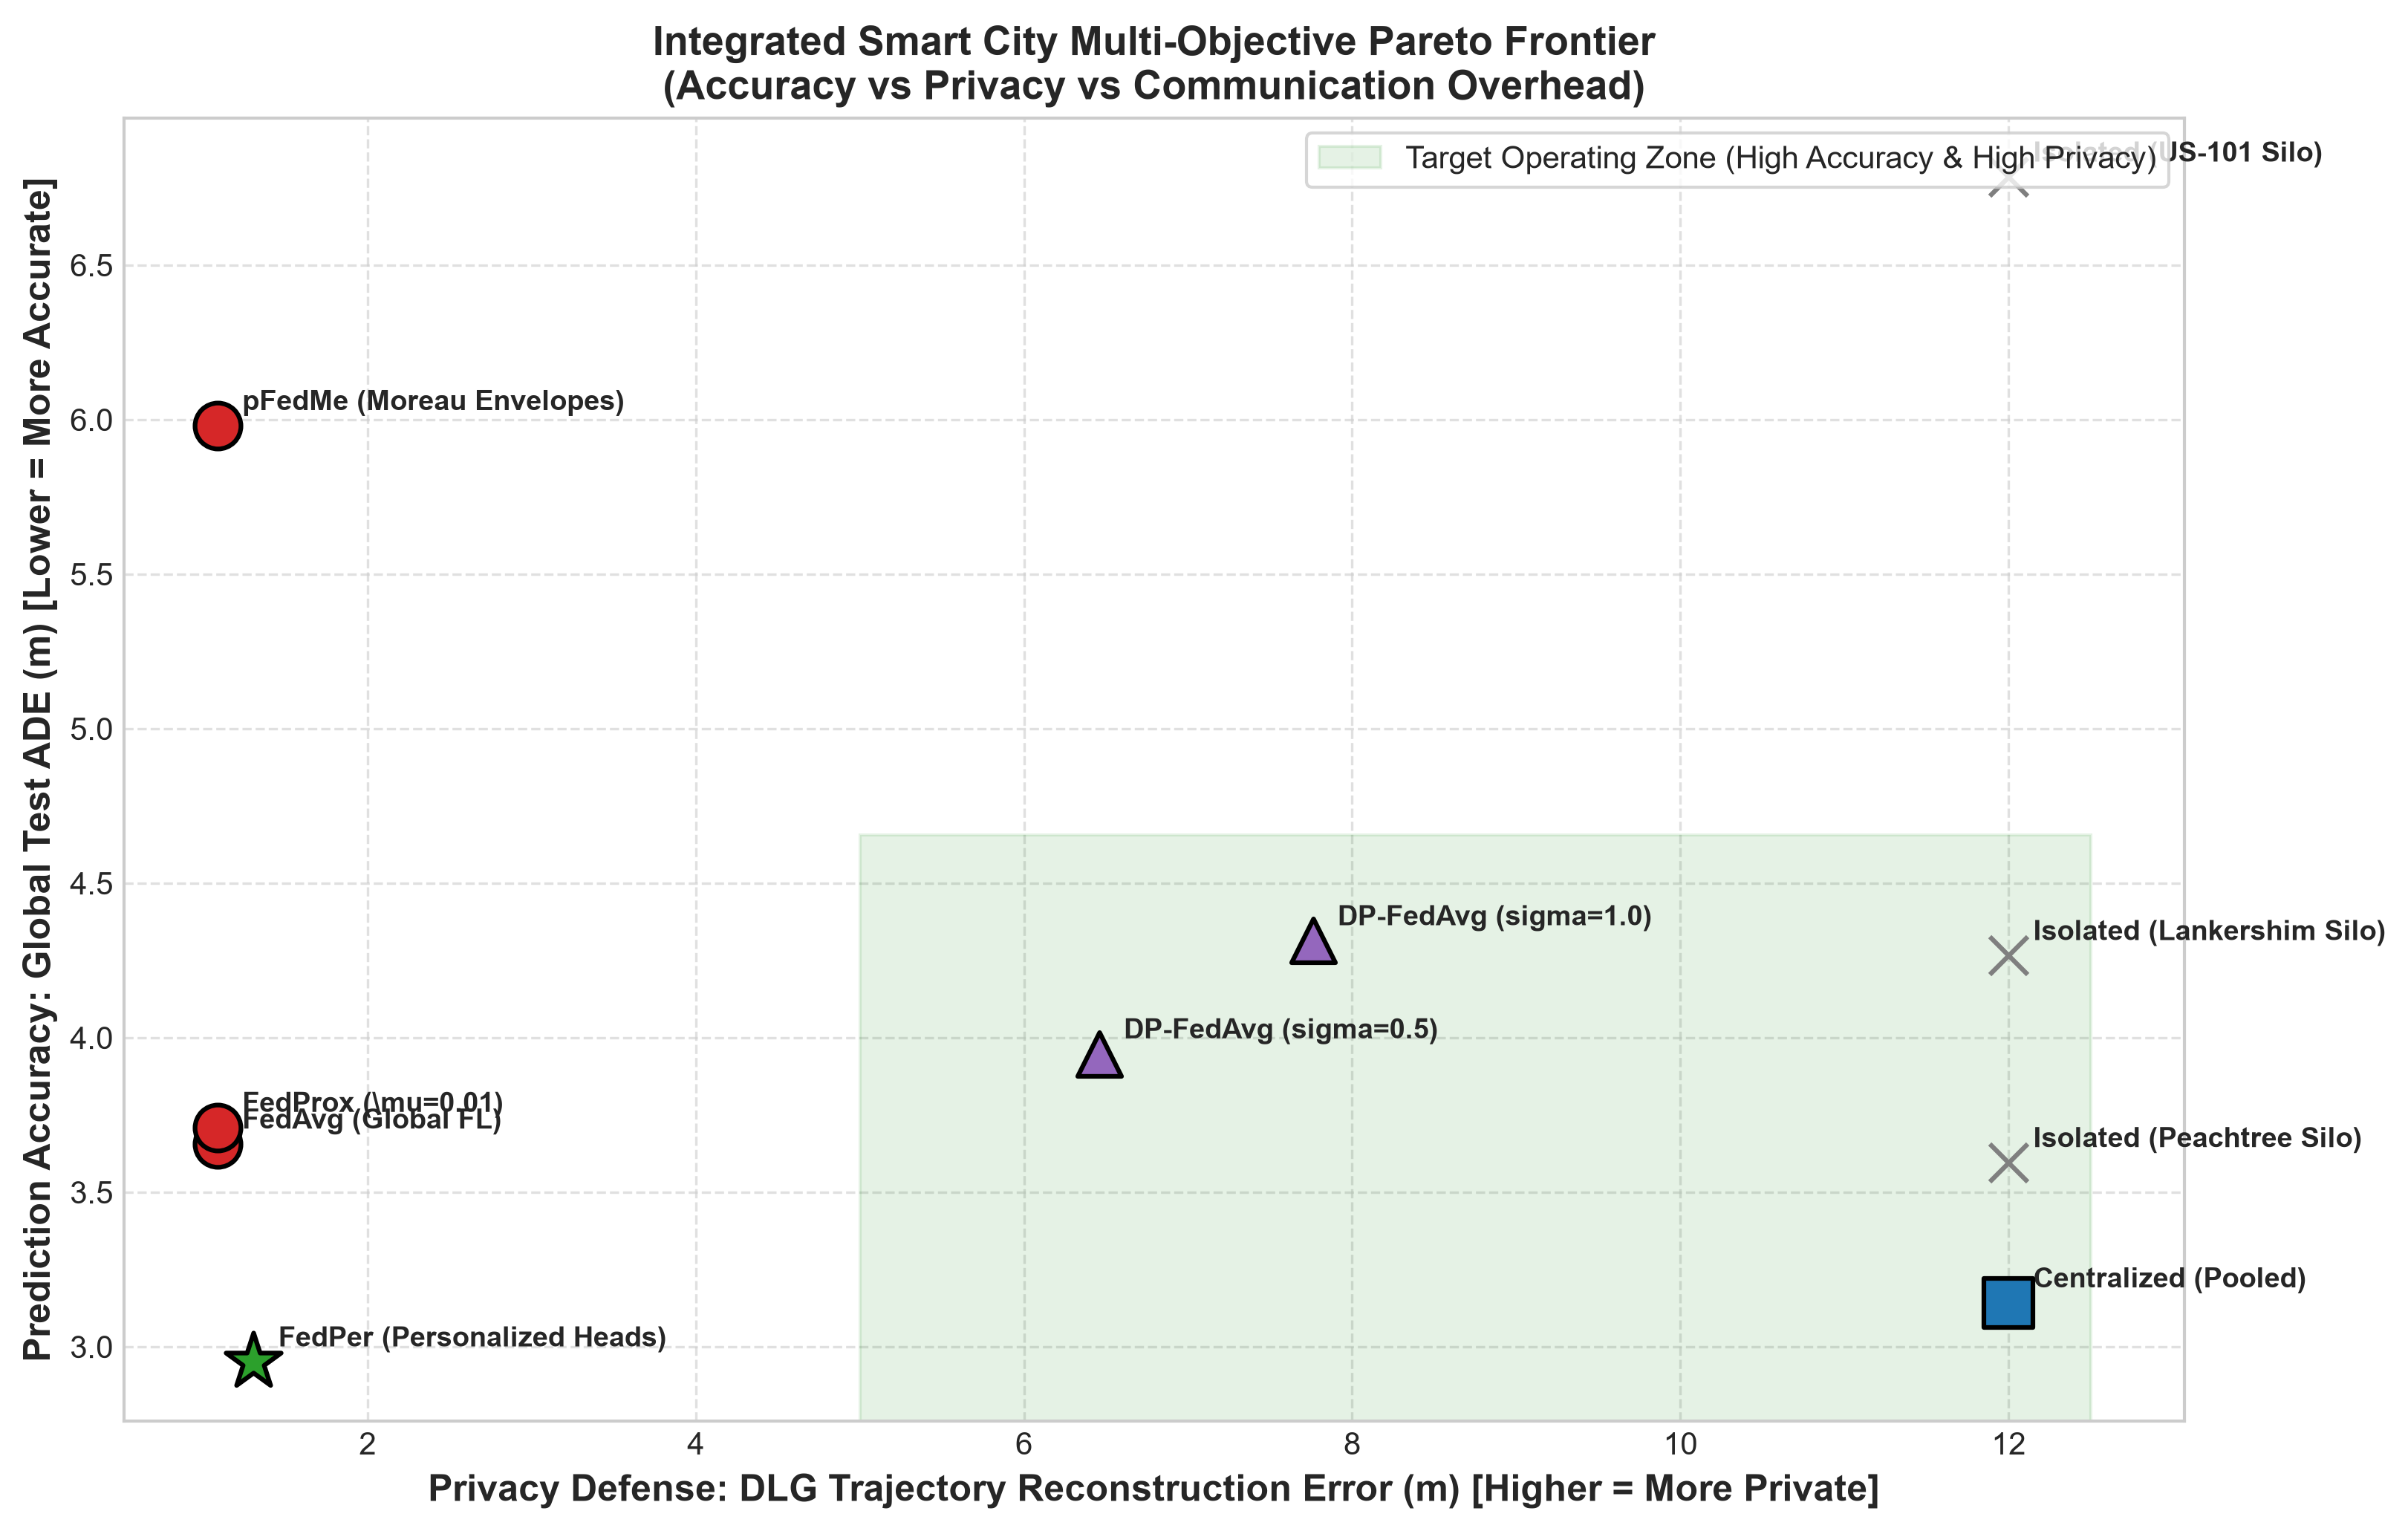
\includegraphics[width=\columnwidth]{fig10_pareto_tradeoff_frontier.png}
\caption{Multi-objective Pareto trade-off frontier illustrating the optimal operating envelope across prediction accuracy, communication overhead, and privacy guarantees.}
\label{fig:pareto_frontier}
\end{figure}

The Pareto optimization matrix in Table~\ref{tab:pareto} and Fig.~\ref{fig:pareto_frontier} demonstrates that FedPer provides the superior trade-off across global accuracy ($2.951$\,m ADE), low backhaul traffic ($36.65$\,MB), and regional equity ($8.081$\,m disparity gap). Adding DP noise ($\sigma = 0.5, \epsilon = 9.69$) to FedAvg maintained an operational ADE of $3.948$\,m while preventing gradient reconstruction with $6.458$\,m error.

% =========================================================================
% SECTION 5: DISCUSSION
% =========================================================================
\section{Discussion}
\label{sec:discussion}

FedPer achieves superior forecasting accuracy ($2.951$\,m ADE) over centralized pooling ($3.142$\,m ADE) and FedAvg ($3.656$\,m ADE) by decoupling temporal representation learning from localized spatial projection. Trajectory prediction involves two distinct learning phases. First, the network learns temporal motion dynamics, such as velocity persistence and acceleration smoothing, which follow shared physical laws across all vehicles. Second, the network maps hidden sequence representations to 2D coordinate offsets. This mapping depends strictly on local road layouts, speed limits, and signal timing. In centralized pooling and canonical FedAvg, forcing a shared regression head across all zones creates severe gradient conflict. High-speed highway trajectories moving at $32.8$\,ft/s pull gradient updates toward large spatial offsets, while arterial trajectories moving at $7.4$\,ft/s pull them toward small increments. FedPer eliminates this conflict. It synchronizes only the LSTM encoder, Bahdanau attention, and LSTM decoder weights across roadside units. Each edge unit keeps its two-layer MLP head private and trains it exclusively on local data. This architectural split allows each roadside unit to map shared temporal features to its specific local spatial scale.

These results challenge earlier transportation studies that viewed centralized pooled training as an unattainable performance ceiling~\cite{dai2024federated, liu2025trajectory}. Prior evaluations on uniform synthetic traffic observed that federated models consistently underperformed centralized models~\cite{dai2024federated, liu2025trajectory}. In contrast, our findings prove that under real geographic distribution shifts ($\overline{\mathrm{JSD}} = 0.1088$), centralized pooling acts as an unweighted compromise that degrades localized accuracy. Our empirical outcomes support Arivazhagan \textit{et al.}~\cite{arivazhagan2019federated}, who demonstrated that separating representation backbones from local heads overcomes non-IID degradation. Our findings also align with Tan \textit{et al.}~\cite{tan2024clustered}, who noted that unified global models diverge when client data distributions differ widely. Furthermore, our privacy audits corroborate the risks identified by Zhu \textit{et al.}~\cite{zhu2019deep} and Zhao \textit{et al.}~\cite{zhao2020idlg}. When roadside units transmit unprotected gradients, an attacker optimizing dummy inputs via L-BFGS to minimize $\|\nabla W_{\mathrm{dummy}} - \nabla W_{\mathrm{real}}\|^2$ reconstructs raw vehicle trajectories within $1.086$\,m error. Isolating output heads under FedPer removes direct output gradient matching, mitigating reconstruction vulnerability.

These findings yield concrete architectural guidelines for roadside intelligent transportation infrastructure. Roadside units operate over cellular backhaul channels with constrained bandwidth budgets and strict privacy regulations. FedPer reduces total uploaded data by $96.08\%$ relative to raw coordinate transmission ($36.65$\,MB compared to $937.29$\,MB). In each communication round, a roadside unit transmits only $521.25$\,KB of base network parameters across the network. Furthermore, because local prediction heads remain on edge devices, coordinate projection weights never leave the local roadside unit. When municipal transport operators mandate rigorous mathematical privacy guarantees, they can incorporate DP-SGD~\cite{abadi2016deep}. By clipping per-sample gradients to $C$ via $g / \max(1, \|g\|_2 / C)$ and injecting calibrated Gaussian noise $\mathcal{N}(0, \sigma^2 C^2 I)$ with $\sigma = 0.5$ ($\epsilon = 9.69$), the edge system suppresses gradient inversion attacks while preserving practical forecasting utility ($3.948$\,m ADE).

This study is subject to three practical limitations. First, the NGSIM trajectory dataset was collected under daylight conditions and fair weather using static overhead cameras. It does not reflect adverse weather conditions, dense fog, sensor occlusions, or sensor calibration drift. Second, our experimental design assumes reliable synchronous communication rounds across all roadside units. In real smart city deployments, edge units experience intermittent packet loss, communication dropouts, and straggler delays. Third, our model forecasts single-vehicle trajectories independently without incorporating multi-agent graph attention matrices. Integrating spatial-temporal graph neural networks to model surrounding vehicle interactions would capture collision avoidance dynamics, but would also increase computational load on edge hardware.

% =========================================================================
% SECTION 6: CONCLUSION
% =========================================================================
\section{Conclusion}
\label{sec:conclusion}
This study evaluated the impact of geographic non-IID data distributions on federated vehicle trajectory forecasting across distributed roadside edge units. Using one million trajectory points from the NGSIM benchmark, we measured empirical kinematic shifts across freeway, arterial, and downtown corridors. We demonstrated that canonical federated averaging suffered from severe client drift and wide regional accuracy disparities. Furthermore, isolated roadside models failed to generalize when evaluated outside their training domains. We showed that personalized federated learning using FedPer overcame these challenges. By sharing a sequence-to-sequence LSTM attention backbone while retaining private local prediction heads, FedPer achieved a global average displacement error of 2.951 meters. This performance surpassed centralized pooled training at 3.142 meters and federated averaging at 3.656 meters. FedPer reduced the regional disparity gap between corridors by 32.7 percent and cut network backhaul communication by 96.08 percent compared to raw coordinate streaming. Privacy audits revealed that unprotected gradient exchanges leaked vehicle trajectories within 1.086 meters of ground truth, whereas prediction head isolation and differential privacy noise eliminated coordinate recovery. Future research investigates asynchronous federated optimization, communication dropouts, and multi-vehicle spatial-temporal graph models.

% =========================================================================
% DECLARATIONS
% =========================================================================
\section*{Declarations}

\subsection*{Acknowledgements}
The author expresses sincere gratitude to the Federal Highway Administration (FHWA) for making the Next Generation Simulation (NGSIM) vehicular trajectory dataset publicly accessible for scientific transportation research.

\subsection*{Funding}
This research received no specific grant from any funding agency in the public, commercial, or not-for-profit sectors.

\subsection*{Conflict of Interest}
The authors declare no conflict of interest.

\subsection*{Data Availability}
The Next Generation Simulation (NGSIM) dataset is publicly available from the Federal Highway Administration (FHWA) at \url{https://ops.fhwa.dot.gov/trafficanalysistools/ngsim.htm}. The code, benchmark evaluation scripts, and experimental result matrices generated in this study are available from the corresponding author upon reasonable request.

\subsection*{Author Contributions}
\textbf{Smit Patel}: Conceptualisation, Methodology, Software, Validation, Formal analysis, Investigation, Writing --- original draft, Writing --- review and editing.

% =========================================================================
% REFERENCES
% =========================================================================
\bibliographystyle{IEEEtran}
\bibliography{references}

\end{document}
